\documentclass[11pt]{article}

\usepackage[usenames,dvipsnames]{xcolor}
\definecolor{Gred}{RGB}{219, 50, 54}
\definecolor{ToCgreen}{RGB}{0, 128, 0}

\usepackage[toc,page]{appendix}
\usepackage{hyperref}
\usepackage{tikz}
\hypersetup{
  colorlinks=true,
  citecolor=ToCgreen,
  linkcolor=Sepia,
  filecolor=Gred,
  urlcolor=Gred
  }

\usepackage{graphicx} % Required for inserting images.
\usepackage[margin=1in]{geometry}
\usepackage{float}
\usepackage{amsmath, amsthm}
\usepackage{mathtools}
\mathtoolsset{showonlyrefs}
\usepackage{verbatim}
\usepackage[numbers]{natbib}
\usepackage{url}            % simple URL typesetting
\usepackage{booktabs}       % professional-quality tables
\usepackage{nicefrac}       % compact symbols for 1/2, etc.
\usepackage{microtype}      % microtypography
\usepackage{multicol}
\usepackage{caption}
\usepackage{enumitem}
\usepackage{mathtools}
\usepackage{thm-restate}
\usepackage[most]{tcolorbox}
\newtheorem{definition}{Definition}
\newtheorem{proposition}{Proposition}
\newtheorem{remark}{Remark}
\newtheorem{theorem}{Theorem}
\newtheorem{assumption}{Assumption}
\newtheorem{example}{Example}
\newtheorem{corollary}{Corollary}
\newtheorem{lemma}[theorem]{Lemma}
\usepackage{subcaption} 
\usepackage[bitstream-charter,cal=cmcal]{mathdesign}
\usepackage[T1]{fontenc}
\AtBeginEnvironment{tcolorbox}{\small}
\usepackage{ifthen}

\newcommand{\I}{\mathbf{I}}
\newcommand{\TV}{\mathrm{TV}}
\newcommand{\KL}{\mathrm{KL}}
\newcommand{\supp}{\mathrm{supp}}
\newcommand{\Hellinger}{\mathrm{H}}
\newcommand{\LC}{\mathrm{LC}}
\newcommand{\Wtwo}{\mathrm{W}_2}
\newcommand{\subsetfunc}{\textrm{Subset}}
\newcommand{\noiseamount}{\textrm{NoiseAmount}}
\newcommand{\sigmamin}
{\sigma^2_{\mathrm{min}}}
\newcommand{\sigmamax}{\sigma^2_{\mathrm{max}}}
\newcommand{\SLC}{\mathrm{SLC}}
\newcommand{\subG}{\mathrm{subG}}
\newcommand{\Sinit}{S_{\mathrm{init}}}
\newcommand{\Send}{S_{\mathrm{target}}}
\newcommand{\Sbefore}{S_{\mathrm{before}}}
\newcommand{\Safter}{S_{\mathrm{after}}}


\newcommand{\wh}{\widehat}



\newcommand{\shortleft}{\scriptscriptstyle\leftarrow}
\newcommand{\shortright}{\scriptscriptstyle\rightarrow}
\newcommand{\orig}{\mathrm{orig}}
\newcommand{\Cat}{\text{Cat}}
\newcommand{\Unif}{\text{Unif}}
\newcommand{\E}{\mathbb{E}}
\newcommand{\R}{\mathbb{R}}
\newcommand{\Z}{\mathbb{Z}}
\newcommand{\D}{\mathrm{d}}
\newcommand{\V}{\mathcal{V}}
\newcommand{\thinshellc}{c}
\newcommand{\thinshellC}{C}
\newcommand{\forward}{X}
\newcommand{\kernelforward}[1][]{%
    \ifthenelse{\equal{#1}{}}%
        {P^{\shortright}}% If no argument is provided
        {P^{\shortright,#1}}% If an argument is provided
}
\newcommand{\kernelreverse}[1][]{%
    \ifthenelse{\equal{#1}{}}%
        {P^{\shortleft}}% If no argument is provided
        {P^{\shortleft,#1}}% If an argument is provided
}
\newcommand{\revsub}[1]{Y^{\shortleft,#1}}
\newcommand{\pathrev}[1]{P^{\shortleft,#1}}
\newcommand{\modrev}[3]
{Y^{\shortleft}_{#3}[#1^{\langle #2\rangle}]}
\newcommand{\reverse}{X^{\shortleft}}
\newcommand{\modrevX}[2]{X^{\shortleft}[#1^{\langle #2\rangle}]}
\newcommand{\modrevpath}[2]{P^{\shortleft}[#1^{\langle #2\rangle}]}
\newcommand{\Id}{\mathrm{Id}}
\newcommand{\calN}{\mathcal{N}}
\newcommand{\alt}{\mathrm{alt}}
\newcommand{\norm}[1]{\|#1\|}
\newcommand{\sitan}[1]{{\color{red} [sitan: #1]}}
\newcommand{\marvin}[1]{{\color{blue} [marvin: #1]}}
\newcommand{\Tupper}{T_{\mathrm{start}}}
\newcommand{\Tlower}{T_{\mathrm{end}}}
\newcommand{\Tbefore}{T_{\mathrm{before}}}
\newcommand{\Tafter}{T_{\mathrm{after}}}


\newcommand{\modrevlaw}[3]{\ifthenelse{\equal{#3}{}}{p^{#1,#2}}{p_{#3}^{#1,#2}}}
\newcommand{\modrevlawX}[2]{p^{#1,#2}}

\newcommand{\llamainstruct}{LLAMA-$3.1$-$8$B-Instruct}
\newcommand{\qweninstruct}{Qwen-$2.5$-$7$B-Instruct}
\newcommand{\phiinstruct}{Phi-$3$-$7$B-Instruct}

\title{Blink of an eye: a simple theory for feature localization in generative models}


\author{
    Marvin Li\thanks{Email:
    \texttt{marvinli@college.harvard.edu}} \\
    Harvard College
    \and
    Aayush Karan\thanks{Email: \texttt{akaran1@g.harvard.edu}, supported in part by the PD Soros fellowship} \\
    Harvard SEAS
    \and
    Sitan Chen\thanks{Email: \texttt{sitan@seas.harvard.edu}, supported in part by NSF Award 2331831} \\
    Harvard SEAS
}

\begin{document}

\maketitle
\begin{abstract}
    \begin{abstract}  
Test time scaling is currently one of the most active research areas that shows promise after training time scaling has reached its limits.
Deep-thinking (DT) models are a class of recurrent models that can perform easy-to-hard generalization by assigning more compute to harder test samples.
However, due to their inability to determine the complexity of a test sample, DT models have to use a large amount of computation for both easy and hard test samples.
Excessive test time computation is wasteful and can cause the ``overthinking'' problem where more test time computation leads to worse results.
In this paper, we introduce a test time training method for determining the optimal amount of computation needed for each sample during test time.
We also propose Conv-LiGRU, a novel recurrent architecture for efficient and robust visual reasoning. 
Extensive experiments demonstrate that Conv-LiGRU is more stable than DT, effectively mitigates the ``overthinking'' phenomenon, and achieves superior accuracy.
\end{abstract}  
\end{abstract}

\newpage

\tableofcontents

\newpage

\section{Introduction}


\begin{figure}[t]
\centering
\includegraphics[width=0.6\columnwidth]{figures/evaluation_desiderata_V5.pdf}
\vspace{-0.5cm}
\caption{\systemName is a platform for conducting realistic evaluations of code LLMs, collecting human preferences of coding models with real users, real tasks, and in realistic environments, aimed at addressing the limitations of existing evaluations.
}
\label{fig:motivation}
\end{figure}

\begin{figure*}[t]
\centering
\includegraphics[width=\textwidth]{figures/system_design_v2.png}
\caption{We introduce \systemName, a VSCode extension to collect human preferences of code directly in a developer's IDE. \systemName enables developers to use code completions from various models. The system comprises a) the interface in the user's IDE which presents paired completions to users (left), b) a sampling strategy that picks model pairs to reduce latency (right, top), and c) a prompting scheme that allows diverse LLMs to perform code completions with high fidelity.
Users can select between the top completion (green box) using \texttt{tab} or the bottom completion (blue box) using \texttt{shift+tab}.}
\label{fig:overview}
\end{figure*}

As model capabilities improve, large language models (LLMs) are increasingly integrated into user environments and workflows.
For example, software developers code with AI in integrated developer environments (IDEs)~\citep{peng2023impact}, doctors rely on notes generated through ambient listening~\citep{oberst2024science}, and lawyers consider case evidence identified by electronic discovery systems~\citep{yang2024beyond}.
Increasing deployment of models in productivity tools demands evaluation that more closely reflects real-world circumstances~\citep{hutchinson2022evaluation, saxon2024benchmarks, kapoor2024ai}.
While newer benchmarks and live platforms incorporate human feedback to capture real-world usage, they almost exclusively focus on evaluating LLMs in chat conversations~\citep{zheng2023judging,dubois2023alpacafarm,chiang2024chatbot, kirk2024the}.
Model evaluation must move beyond chat-based interactions and into specialized user environments.



 

In this work, we focus on evaluating LLM-based coding assistants. 
Despite the popularity of these tools---millions of developers use Github Copilot~\citep{Copilot}---existing
evaluations of the coding capabilities of new models exhibit multiple limitations (Figure~\ref{fig:motivation}, bottom).
Traditional ML benchmarks evaluate LLM capabilities by measuring how well a model can complete static, interview-style coding tasks~\citep{chen2021evaluating,austin2021program,jain2024livecodebench, white2024livebench} and lack \emph{real users}. 
User studies recruit real users to evaluate the effectiveness of LLMs as coding assistants, but are often limited to simple programming tasks as opposed to \emph{real tasks}~\citep{vaithilingam2022expectation,ross2023programmer, mozannar2024realhumaneval}.
Recent efforts to collect human feedback such as Chatbot Arena~\citep{chiang2024chatbot} are still removed from a \emph{realistic environment}, resulting in users and data that deviate from typical software development processes.
We introduce \systemName to address these limitations (Figure~\ref{fig:motivation}, top), and we describe our three main contributions below.


\textbf{We deploy \systemName in-the-wild to collect human preferences on code.} 
\systemName is a Visual Studio Code extension, collecting preferences directly in a developer's IDE within their actual workflow (Figure~\ref{fig:overview}).
\systemName provides developers with code completions, akin to the type of support provided by Github Copilot~\citep{Copilot}. 
Over the past 3 months, \systemName has served over~\completions suggestions from 10 state-of-the-art LLMs, 
gathering \sampleCount~votes from \userCount~users.
To collect user preferences,
\systemName presents a novel interface that shows users paired code completions from two different LLMs, which are determined based on a sampling strategy that aims to 
mitigate latency while preserving coverage across model comparisons.
Additionally, we devise a prompting scheme that allows a diverse set of models to perform code completions with high fidelity.
See Section~\ref{sec:system} and Section~\ref{sec:deployment} for details about system design and deployment respectively.



\textbf{We construct a leaderboard of user preferences and find notable differences from existing static benchmarks and human preference leaderboards.}
In general, we observe that smaller models seem to overperform in static benchmarks compared to our leaderboard, while performance among larger models is mixed (Section~\ref{sec:leaderboard_calculation}).
We attribute these differences to the fact that \systemName is exposed to users and tasks that differ drastically from code evaluations in the past. 
Our data spans 103 programming languages and 24 natural languages as well as a variety of real-world applications and code structures, while static benchmarks tend to focus on a specific programming and natural language and task (e.g. coding competition problems).
Additionally, while all of \systemName interactions contain code contexts and the majority involve infilling tasks, a much smaller fraction of Chatbot Arena's coding tasks contain code context, with infilling tasks appearing even more rarely. 
We analyze our data in depth in Section~\ref{subsec:comparison}.



\textbf{We derive new insights into user preferences of code by analyzing \systemName's diverse and distinct data distribution.}
We compare user preferences across different stratifications of input data (e.g., common versus rare languages) and observe which affect observed preferences most (Section~\ref{sec:analysis}).
For example, while user preferences stay relatively consistent across various programming languages, they differ drastically between different task categories (e.g. frontend/backend versus algorithm design).
We also observe variations in user preference due to different features related to code structure 
(e.g., context length and completion patterns).
We open-source \systemName and release a curated subset of code contexts.
Altogether, our results highlight the necessity of model evaluation in realistic and domain-specific settings.





\section{Preliminaries}
\label{sec:prelim}
\label{sec:term}
We define the key terminologies used, primarily focusing on the hidden states (or activations) during the forward pass. 

\paragraph{Components in an attention layer.} We denote $\Res$ as the residual stream. We denote $\Val$ as Value (states), $\Qry$ as Query (states), and $\Key$ as Key (states) in one attention head. The \attlogit~represents the value before the softmax operation and can be understood as the inner product between  $\Qry$  and  $\Key$. We use \Attn~to denote the attention weights of applying the SoftMax function to \attlogit, and ``attention map'' to describe the visualization of the heat map of the attention weights. When referring to the \attlogit~from ``$\tokenB$'' to  ``$\tokenA$'', we indicate the inner product  $\langle\Qry(\tokenB), \Key(\tokenA)\rangle$, specifically the entry in the ``$\tokenB$'' row and ``$\tokenA$'' column of the attention map.

\paragraph{Logit lens.} We use the method of ``Logit Lens'' to interpret the hidden states and value states \citep{belrose2023eliciting}. We use \logit~to denote pre-SoftMax values of the next-token prediction for LLMs. Denote \readout~as the linear operator after the last layer of transformers that maps the hidden states to the \logit. 
The logit lens is defined as applying the readout matrix to residual or value states in middle layers. Through the logit lens, the transformed hidden states can be interpreted as their direct effect on the logits for next-token prediction. 

\paragraph{Terminologies in two-hop reasoning.} We refer to an input like “\Src$\to$\brga, \brgb$\to$\Ed” as a two-hop reasoning chain, or simply a chain. The source entity $\Src$ serves as the starting point or origin of the reasoning. The end entity $\Ed$ represents the endpoint or destination of the reasoning chain. The bridge entity $\Brg$ connects the source and end entities within the reasoning chain. We distinguish between two occurrences of $\Brg$: the bridge in the first premise is called $\brga$, while the bridge in the second premise that connects to $\Ed$ is called $\brgc$. Additionally, for any premise ``$\tokenA \to \tokenB$'', we define $\tokenA$ as the parent node and $\tokenB$ as the child node. Furthermore, if at the end of the sequence, the query token is ``$\tokenA$'', we define the chain ``$\tokenA \to \tokenB$, $\tokenB \to \tokenC$'' as the Target Chain, while all other chains present in the context are referred to as distraction chains. Figure~\ref{fig:data_illustration} provides an illustration of the terminologies.

\paragraph{Input format.}
Motivated by two-hop reasoning in real contexts, we consider input in the format $\bos, \text{context information}, \query, \answer$. A transformer model is trained to predict the correct $\answer$ given the query $\query$ and the context information. The context compromises of $K=5$ disjoint two-hop chains, each appearing once and containing two premises. Within the same chain, the relative order of two premises is fixed so that \Src$\to$\brga~always precedes \brgb$\to$\Ed. The orders of chains are randomly generated, and chains may interleave with each other. The labels for the entities are re-shuffled for every sequence, choosing from a vocabulary size $V=30$. Given the $\bos$ token, $K=5$ two-hop chains, \query, and the \answer~tokens, the total context length is $N=23$. Figure~\ref{fig:data_illustration} also illustrates the data format. 

\paragraph{Model structure and training.} We pre-train a three-layer transformer with a single head per layer. Unless otherwise specified, the model is trained using Adam for $10,000$ steps, achieving near-optimal prediction accuracy. Details are relegated to Appendix~\ref{app:sec_add_training_detail}.


% \RZ{Do we use source entity, target entity, and mediator entity? Or do we use original token, bridge token, end token?}





% \paragraph{Basic notations.} We use ... We use $\ve_i$ to denote one-hot vectors of which only the $i$-th entry equals one, and all other entries are zero. The dimension of $\ve_i$ are usually omitted and can be inferred from contexts. We use $\indicator\{\cdot\}$ to denote the indicator function.

% Let $V > 0$ be a fixed positive integer, and let $\vocab = [V] \defeq \{1, 2, \ldots, V\}$ be the vocabulary. A token $v \in \vocab$ is an integer in $[V]$ and the input studied in this paper is a sequence of tokens $s_{1:T} \defeq (s_1, s_2, \ldots, s_T) \in \vocab^T$ of length $T$. For any set $\mathcal{S}$, we use $\Delta(\mathcal{S})$ to denote the set of distributions over $\mathcal{S}$.

% % to a sequence of vectors $z_1, z_2, \ldots, z_T \in \real^{\dout}$ of dimension $\dout$ and length $T$.

% Let $\mU = [\vu_1, \vu_2, \ldots, \vu_V]^\transpose \in \real^{V\times d}$ denote the token embedding matrix, where the $i$-th row $\vu_i \in \real^d$ represents the $d$-dimensional embedding of token $i \in [V]$. Similarly, let $\mP = [\vp_1, \vp_2, \ldots, \vp_T]^\transpose \in \real^{T\times d}$ denote the positional embedding matrix, where the $i$-th row $\vp_i \in \real^d$ represents the $d$-dimensional embedding of position $i \in [T]$. Both $\mU$ and $\mP$ can be fixed or learnable.

% After receiving an input sequence of tokens $s_{1:T}$, a transformer will first process it using embedding matrices $\mU$ and $\mP$ to obtain a sequence of vectors $\mH = [\vh_1, \vh_2, \ldots, \vh_T] \in \real^{d\times T}$, where 
% \[
% \vh_i = \mU^\transpose\ve_{s_i} + \mP^\transpose\ve_{i} = \vu_{s_i} + \vp_i.
% \]

% We make the following definitions of basic operations in a transformer.

% \begin{definition}[Basic operations in transformers] 
% \label{defn:operators}
% Define the softmax function $\softmax(\cdot): \real^d \to \real^d$ over a vector $\vv \in \real^d$ as
% \[\softmax(\vv)_i = \frac{\exp(\vv_i)}{\sum_{j=1}^d \exp(\vv_j)} \]
% and define the softmax function $\softmax(\cdot): \real^{m\times n} \to \real^{m \times n}$ over a matrix $\mV \in \real^{m\times n}$ as a column-wise softmax operator. For a squared matrix $\mM \in \real^{m\times m}$, the causal mask operator $\mask(\cdot): \real^{m\times m} \to \real^{m\times m}$  is defined as $\mask(\mM)_{ij} = \mM_{ij}$ if $i \leq j$ and  $\mask(\mM)_{ij} = -\infty$ otherwise. For a vector $\vv \in \real^n$ where $n$ is the number of hidden neurons in a layer, we use $\layernorm(\cdot): \real^n \to \real^n$ to denote the layer normalization operator where
% \[
% \layernorm(\vv)_i = \frac{\vv_i-\mu}{\sigma}, \mu = \frac{1}{n}\sum_{j=1}^n \vv_j, \sigma = \sqrt{\frac{1}{n}\sum_{j=1}^n (\vv_j-\mu)^2}
% \]
% and use $\layernorm(\cdot): \real^{n\times m} \to \real^{n\times m}$ to denote the column-wise layer normalization on a matrix.
% We also use $\nonlin(\cdot)$ to denote element-wise nonlinearity such as $\relu(\cdot)$.
% \end{definition}

% The main components of a transformer are causal self-attention heads and MLP layers, which are defined as follows.

% \begin{definition}[Attentions and MLPs]
% \label{defn:attn_mlp} 
% A single-head causal self-attention $\attn(\mH;\mQ,\mK,\mV,\mO)$ parameterized by $\mQ,\mK,\mV \in \real^{{\dqkv\times \din}}$ and $\mO \in \real^{\dout\times\dqkv}$ maps an input matrix $\mH \in \real^{\din\times T}$ to
% \begin{align*}
% &\attn(\mH;\mQ,\mK,\mV,\mO) \\
% =&\mO\mV\layernorm(\mH)\softmax(\mask(\layernorm(\mH)^\transpose\mK^\transpose\mQ\layernorm(\mH))).
% \end{align*}
% Furthermore, a multi-head attention with $M$ heads parameterized by $\{(\mQ_m,\mK_m,\mV_m,\mO_m) \}_{m=1}^M$ is defined as 
% \begin{align*}
%     &\Attn(\mH; \{(\mQ_m,\mK_m,\mV_m,\mO_m) \}_{m\in[M]}) \\ =& \sum_{m=1}^M \attn(\mH;\mQ_m,\mK_m,\mV_m,\mO_m) \in \real^{\dout \times T}.
% \end{align*}
% An MLP layer $\mlp(\mH;\mW_1,\mW_2)$ parameterized by $\mW_1 \in \real^{\dhidden\times \din}$ and $\mW_2 \in \real^{\dout \times \dhidden}$ maps an input matrix $\mH = [\vh_1, \ldots, \vh_T] \in \real^{\din \times T}$ to
% \begin{align*}
%     &\mlp(\mH;\mW_1,\mW_2) = [\vy_1, \ldots, \vy_T], \\ \text{where } &\vy_i = \mW_2\nonlin(\mW_1\layernorm(\vh_i)), \forall i \in [T].
% \end{align*}

% \end{definition}

% In this paper, we assume $\din=\dout=d$ for all attention heads and MLPs to facilitate residual stream unless otherwise specified. Given \Cref{defn:operators,defn:attn_mlp}, we are now able to define a multi-layer transformer.

% \begin{definition}[Multi-layer transformers]
% \label{defn:transformer}
%     An $L$-layer transformer $\transformer(\cdot): \vocab^T \to \Delta(\vocab)$ parameterized by $\mP$, $\mU$, $\{(\mQ_m^{(l)},\mK_m^{(l)},\mV_m^{(l)},\mO_m^{(l)})\}_{m\in[M],l\in[L]}$,  $\{(\mW_1^{(l)},\mW_2^{(l)})\}_{l\in[L]}$ and $\Wreadout \in \real^{V \times d}$ receives a sequence of tokens $s_{1:T}$ as input and predict the next token by outputting a distribution over the vocabulary. The input is first mapped to embeddings $\mH = [\vh_1, \vh_2, \ldots, \vh_T] \in \real^{d\times T}$ by embedding matrices $\mP, \mU$ where 
%     \[
%     \vh_i = \mU^\transpose\ve_{s_i} + \mP^\transpose\ve_{i}, \forall i \in [T].
%     \]
%     For each layer $l \in [L]$, the output of layer $l$, $\mH^{(l)} \in \real^{d\times T}$, is obtained by 
%     \begin{align*}
%         &\mH^{(l)} =  \mH^{(l-1/2)} + \mlp(\mH^{(l-1/2)};\mW_1^{(l)},\mW_2^{(l)}), \\
%         & \mH^{(l-1/2)} = \mH^{(l-1)} + \\ & \quad \Attn(\mH^{(l-1)}; \{(\mQ_m^{(l)},\mK_m^{(l)},\mV_m^{(l)},\mO_m^{(l)}) \}_{m\in[M]}), 
%     \end{align*}
%     where the input $\mH^{(l-1)}$ is the output of the previous layer $l-1$ for $l > 1$ and the input of the first layer $\mH^{(0)} = \mH$. Finally, the output of the transformer is obtained by 
%     \begin{align*}
%         \transformer(s_{1:T}) = \softmax(\Wreadout\vh_T^{(L)})
%     \end{align*}
%     which is a $V$-dimensional vector after softmax representing a distribution over $\vocab$, and $\vh_T^{(L)}$ is the $T$-th column of the output of the last layer, $\mH^{(L)}$.
% \end{definition}



% For each token $v \in \vocab$, there is a corresponding $d_t$-dimensional token embedding vector $\embed(v) \in \mathbb{R}^{d_t}$. Assume the maximum length of the sequence studied in this paper does not exceed $T$. For each position $t \in [T]$, there is a corresponding positional embedding  










\section{Characterization of critical windows}\label{sec:master}

Let $\Sinit\subset\Theta$ denote some sub-mixture, corresponding to a sub-population of $p$ that possesses a certain property. For instance, if $p$ corresponds to some autoregressive model, $\Sinit$ might correspond to sentences which correctly answer a particular math question. Let $\Send\supset\Sinit$ denote some sub-mixture containing $\Sinit$. For instance, $\Send$ might correspond to all possible responses to the math question, including incorrect ones.

We are interested in the following question: if we run the forward-reverse experiment for time $\wh{T}$ starting from $p^{\Sinit}$, is there some range of times for which the resulting distribution is close to $p^{\Send}$? That is, can we characterize the $\wh{T}$ for which
\begin{equation}
    \TV(\modrevlaw{\Sinit}{\wh{T}}{}, p^{\Send})
\end{equation}
is small?

Suppose one could prove that the range of $\wh{T}$ for which this is the case is some interval $[T_0, T_1]$. This would mean that if the stochastic localization sampler runs for time $T$ and ends up at a sample from $p^{\Sinit}$, then from time $T - T_1$ to time $T - T_0$ of the generation process, \emph{the sampler has not yet localized the features that distinguish $p^{\Sinit}$ from the larger sub-mixture $p^{\Send}$}. However, the sampler has localized the features that distinguish $p^{\Send}$ from $p^{\Theta-\Send}$. When there is a shift from localizing the features $\Send$ to the features $\Sinit$, we say there is a critical window. We now formally state and prove our main result.  

\subsection{Main result} 

For an error parameter $0 < \epsilon < 1$, define
\begin{align*} 
\Tupper(\epsilon) \in \sup\{&t \in \I:\TV(p_{t}^{\Send}  ,p_{t}^{\Theta-\Send }) \geq 1-\epsilon^2\,\} \\
\Tlower(\epsilon) \in  \inf\{&t \in  \I:  \TV(p_{t}^{S_{\mathrm{init}}  },p_{t}^{\Send }) \leq \epsilon\}\,.
\end{align*} 
This is well-defined for continuous observation processes.\footnote{For general stochastic localization schemes, we can only ask that $\Tupper(\epsilon) \in  \{ r\in \I:\TV(p_{t}^{\Send} ,p_{t}^{\Theta-\Send }) \geq 1-\epsilon^2\,\}$ and $\Tlower(\epsilon) \in  \{t \in  \I:  \TV(p_{t}^{S_{\mathrm{init}}  },p_{t}^{\Send }) \leq \epsilon\}$ instead of $\sup,\inf$ like \citep{li2024criticalwindowsnonasymptotictheory}, because the sets $ \{t \in \I:\TV(p_{t}^{\Send}  ,p_{t}^{\Theta-\Send }) \geq 1-\epsilon^2\,\},\{t \in  \I:  \TV(p_{t}^{S_{\mathrm{init}}  },p_{t}^{\Send }) \leq \epsilon\}$ may not be closed for observation processes which are discontinuous. For autoregressive language models and continuous diffusion, the observation process is continuous, so we will elide these technicalities.
.} When the value of $\epsilon$ is understood, we abbreviate the above with $\Tupper$ and $\Tlower$.  Our main result is that in $\wh{T}\in \I \cap [\Tlower,\Tupper]$, the distance $\TV(\modrevlaw{\Sinit}{\wh{T}}{}, p^{\Send})$ is small:

\begin{theorem}\label{thm:masters_theorem} 
Let $S_{\mathrm{init}}\subset \Send \subset \Theta$ and $W=\frac{\sum_{\theta \in \Theta-\Send} w_\theta}{\sum_{\theta \in \Send} w_\theta}$. For $\epsilon > 0$, if $\wh{T}\in \I \cap [\Tlower,\Tupper]$, then  
$\TV(\modrevlaw{\Sinit}{\wh{T}}{}, p^{\Send}) \leq \epsilon\cdot\bigl(1+\max\left(1,W\right)/\sqrt{2}\bigr).$
\end{theorem}
Intuitively, $\Tupper$ represents the largest $t$ for which there is still separation between $\Send$ and $\Theta-\Send$, and $\Tlower$ represents the smallest $t$ for which samples from $\Sinit,\Send$ are indistinguishable. Thus, running it for $\wh{T}\in \I \cap [\Tlower,\Tupper]$ erases the differences between samples from $\Sinit$ and $\Send$ but preserves the difference between $\Send$ and $\Theta-\Send$, yielding samples looking like $p^{\Send}$.
\begin{remark}
\emph{A priori} it is not clear why $\Tlower$ should be smaller than $\Tupper$, and indeed in general it need not be and our bound would be vacuous. In Section~\ref{sec:eg_theory} however, we show that in many natural settings for diffusion models and autoregressive models, the relation does hold.
\end{remark}
\begin{remark}
Note a similar bound was shown in the context of diffusions by \cite{li2024criticalwindowsnonasymptotictheory} (see Theorem 7 therein), who used an approximation argument from~\cite{DBLP:conf/iclr/ChenC0LSZ23} and Girsanov's theorem to prove thei results. Our result is a strict improvement of that bound along several important axes. First, our results apply to all stochastic localization samplers, not just diffusions. This is because our proof is extremely simple and does not require any stochastic calculus. Secondly, \cite{li2024criticalwindowsnonasymptotictheory} needed to assume that the components of $p$ were strongly log-concave and that the score, i.e. gradient of the log-density, of $p_t$ was Lipschitz and moment-bounded for all $t$. Thirdly, their final bound includes a polynomial dependence on the moments of the score, which scale with the dimension $d$; in contrast, our final bound is independent of $d$. 

\end{remark}

With Theorem~\ref{thm:masters_theorem} in place, we are ready to formally define \emph{critical windows}. These capture the moments where we transition from sampling from a sub-mixture to a subset of that sub-mixture.
\begin{definition}
Define $\Safter \subset \Sbefore \subset \Theta$. For $\Sbefore$, we define $\Tbefore =\inf\{t \in \I:\TV(p_t^{\Safter},p_t^{\Sbefore}) \leq \epsilon \text{ and } \TV(p_t^{\Sbefore},p_t^{\Theta-\Sbefore})\geq 1- \epsilon^2\}$ ($\Sinit\triangleq \Safter;\Send\triangleq \Sbefore)$. For $\Safter$, consider $\Tafter = \sup \{t \in \I:\TV(p_t^{\Safter},p_t^{\Theta-\Safter}) \geq 1-\epsilon^2\}$ ($\Sinit,\Send\triangleq\Safter$). A \textbf{critical window} is the interval $[\Tafter,\Tbefore]$, where there is a transition from sampling from $\Sbefore$ to the smaller subset $\Safter$. 
\end{definition}
\begin{figure}[H]
\centering
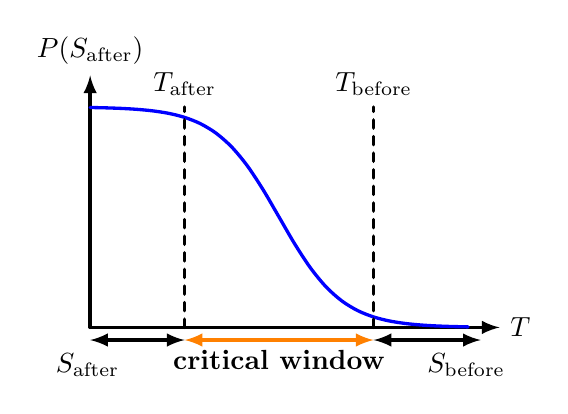
\begin{tikzpicture}[>=latex, line cap=round, scale=0.8,line join=round]
% Axes
\draw[->,very thick] (0,0) -- (6.5,0) node[right] {$T$};
\draw[->,very thick] (0,0) -- (0,4) node[above] {$P(S_{\text{after}})$};

% Probability curve
\draw[very thick,domain=0:6,smooth,variable=\x,color=blue] 
    plot ({\x}, {3.5/(1+exp(2*(\x-3)))});

% Vertical dashed lines
\draw[dashed,very thick] (1.5,0) -- (1.5,3.5);
\draw[dashed,very thick] (4.5,0) -- (4.5,3.5);

% Labels for T_after and T_before
\node[below] at (1.5,4.2) {$T_{\text{after}}$};
\node[below] at (4.5,4.2) {$T_{\text{before}}$};

% Horizontal annotation for critical interval
\draw[<->,very thick] (0,-0.2) -- (1.5,-0.2);
\node[right] at (-0.7,-0.6) {$\Safter$};

\draw[<->,very thick,color=orange] (1.5,-0.2) -- (4.5,-0.2);
\node[below] at (3,-0.2) {\textbf{critical window}};

\draw[<->,very thick] (4.5,-0.2) -- (6.2,-0.2);
\node[right] at (5.2,-0.6) {$\Sbefore$};
\end{tikzpicture}
\caption{Illustration of the definition of a critical window for a simple mixture of two Gaussians, with $\Sbefore\triangleq\{\mathcal{N}(\mu,\mathrm{Id}),\mathcal{N}(-\mu,\mathrm{Id})\}$ and $\Safter\triangleq\{\mathcal{N}(\mu,\mathrm{Id})\}$.}
\label{fig:cw_definition}
\end{figure}
For nonempty $S \subset \Theta$ and $t \in \I$, we define $\kernelreverse[](\cdot |Y_t,S)$ to be the posterior of $X$ with the prior $X \sim p^S$. We similarly define $\kernelreverse[]_{t \to \Theta}(\cdot | Y_t)$ and $\kernelreverse[]_{t \to \Theta}(\cdot | Y_t,S)$ to be the posterior of $\theta$ conditioning on $Y_{t}$ with $X \sim p$ or $X \sim p^S$, respectively. When $S=\{i\}$, we exclude the braces.
\subsection{Proof of Theorem~\ref{thm:masters_theorem}}

\noindent Crucially, our proof relies in several places on the Markov property of stochastic localization samplers, together with the data processing inequality. 

\begin{proof}[Proof of Theorem~\ref{thm:masters_theorem}]
By the triangle inequality, we can write
\begin{align*}
\TV(\modrevlawX{\Sinit}{\wh{T}},p^{\Send})\leq \underbrace{\TV(\modrevlawX{\Sinit}{\wh{T}},\modrevlawX{\Send}{\wh{T}})}_{\text{(I)}}+\underbrace{\TV(\modrevlawX{\Send}{\wh{T}},p^{\Send})}_{\text{(II)}}.
\end{align*}
$\modrevlawX{\Sinit}{\wh{T}}$ and $\modrevlawX{\Send}{\wh{T}}$ are the laws of the posterior $\kernelreverse[](\cdot | \cdot)$ but applied to $Y_{\wh{T}}$ with distributions $p^{\Sinit}_{\wh{T}}$ and $p^{\Send}_{\wh{T}}$. Using the Markov property of localization-based samplers (Definition~\ref{def:observation_process}), we apply the data processing inequality twice and the definition of $\Tlower$ to bound (I) via \[\TV(\modrevlawX{\Sinit}{\wh{T}},\modrevlawX{\Send}{\wh{T}})\leq \TV(p^{S_{\mathrm{init}}  }_{\wh{T}},p^{\Send}_{\wh{T}}) 
 \leq\TV(p^{S_{\mathrm{init}}  }_{\Tlower},p^{\Send}_{\Tlower}) \leq \epsilon.
\]

To bound (II), we use the definition of $\TV$ and a coupling argument. Observe that the observation processes associated with $\modrevlawX{\Send}{\wh{T}}$ and $p^{\Send}$ have the same distribution at index $\wh{T}$. Thus, taking $Y_{\wh{T}} \sim p^{\Send}_{\wh{T}}$, we can express by the law of total probability,
\begin{align*}
\modrevlawX{\Send}{\wh{T}}(x)&=\E[\kernelreverse[](x| Y_{\wh{T}})]\\
p^{\Send}(x)&=\E[\kernelreverse[](x| Y_{\wh{T}},\Send)].
\end{align*}
as these observation processes have the same distribution at index $\wh{T}$. Thus, 
\begin{align*}
\TV(\modrevlawX{\Send}{\wh{T}},p^{\Send}) = \frac{1}{2}  \int \left|\modrevlawX{\Send}{\wh{T}}(x)-p^{\Send}(x) \right|dx=\frac{1}{2} \int \left| \E[\kernelreverse[](x| Y_{\wh{T}})] -\E[\kernelreverse[](x| Y_{\wh{T}},\Send)]. \right|dx.
\end{align*}
By Jensen's inequality and Fubini's theorem, we bring the expectation outside the integral, 
\begin{align*}
\TV(\modrevlawX{\Send}{\wh{T}},p^{\Send}) &\leq \frac{1}{2} \int \E\left[\left|\kernelreverse[](x| Y_{\wh{T}})-\kernelreverse[](x| Y_{\wh{T}},\Send)\right|\right] dx=\frac{1}{2}\E\left[\int \left|\kernelreverse[](x| Y_{\wh{T}})-\kernelreverse[](x| Y_{\wh{T}},\Send)\right| dx\right].
\end{align*}
To simplify the above expression, we use the following two lemmas, proved in App.~\ref{app:master_details}.
\begin{restatable}{lemma}{masterinequality}\label{lem:master_inequality}
By applying the law of total probability and Bayes' rule, we can show for $Y_{\wh{T}}\in\supp(p^{\Send}_{\wh{T}})$,
\begin{align*}
\int \left|\kernelreverse[](x| Y_{\wh{T}})-\kernelreverse[](x| Y_{\wh{T}},\Send)\right| dx \leq  2 \sum_{\theta \in \Theta-\Send} \kernelreverse[]_{t \to \Theta}(\theta|Y_{\wh{T}}).
\end{align*}
\end{restatable} 
\begin{restatable}{lemma}{masterinequalitytwo}\label{lem:master_inequalitytwo}
By Bayes's rule, we can derive for $Y_{\wh{T}} \in \supp(p_{\wh{T}})$,
\begin{align*}
 \sum_{\theta \in \Theta-\Send} \kernelreverse[]_{t \to \Theta}(\theta|Y_{\wh{T}}) \leq  \max\left(1,W\right)  \frac{p^{\Theta-\Send}_{\wh{T}}(Y_{\wh{T}})}{ p^{\Theta-\Send}_{\wh{T}}(Y_{\wh{T}})+p^{\Send}_{\wh{T}}(Y_{\wh{T}})}
\end{align*}
\end{restatable} 
\noindent Combining Lemmas~\ref{lem:master_inequality} and~\ref{lem:master_inequalitytwo} , we find 
\begin{align*}
\TV(\modrevlawX{\Send}{\wh{T}},p^{\Send}) \leq \max\left(1,W\right) \E\left[ \frac{p^{\Theta-\Send}_{\wh{T}}(Y_{\wh{T}})}{ p^{\Theta-\Send}_{\wh{T}}(Y_{\wh{T}})+p^{\Send}_{\wh{T}}(Y_{\wh{T}})}\right]. 
\end{align*}
Then, finally applying Lemma~\ref{lem:ratio_inequality}, we are able to bound the total variation in terms of $\epsilon$, 
\begin{align*}
\TV(\modrevlawX{\Send}{\wh{T}},p^{\Send}) \leq \frac{1}{2}\max\left(1,W\right) \sqrt{1-\TV^2(p^{\Theta-\Send}_{\wh{T}},p^{\Send}_{\wh{T}})}\leq \frac{\sqrt{2}}{2}\max\left(1,W\right) \epsilon.
\end{align*}
\noindent Combining our bounds on (I) and (II) achieves the desired result.
\end{proof}



\begin{figure*}[ht!]
    \centering
    \includegraphics[width=0.99\linewidth]{plots/squares_p4_and_z1z2_d5000_10seeds_overlaps.pdf}
    \caption{Overlap $\normf{\bM}^2 / \Tr(\bQ)$ as a function of the sample complexity $\alpha$. The dots represent numerical simulation results, computed for $n = 5000$ (for the asymmetric method) or $d = 5000$ (for the symmetric method) and averaging over $10$ instances. (\textbf{Left}) Link function $g(z_1,z_2) = z_1z_2$. Solid lines are obtained from state evolution predictions eq. (\ref{eq:overlap_prod_zk},\ref{eq:examples_symmetric_general}). Dashed line at $\alpha_c \approx 0.59375$. (\textbf{Right}) Link function $g(\bz) = p^{-1}\norm{\bz}^2$, $p = 4$. Solid lines are obtained from state evolution predictions eq. (\ref{eq:overlap_asymmetric_squares},\ref{eq:examples_symmetric_general}). Dashed line at $\alpha_c = 2$.}
    \label{fig:z1z2_overlap}
\end{figure*}
In this section we illustrate the framework introduced in Section \ref{sec:main_results} to predict the asymptotic performance of the spectral estimators (\ref{eq:def:spectral_asymmetric},\ref{eq:def:spectral_symmetric}) for specific examples of link functions, providing a comparison between our asymptotic analytical results and finite size numerical simulations for the overlap between the spectral estimators and the weights $\mat{W}_\star$, defined as $m \coloneqq \nicefrac{\normf{\bM}}{\sqrt{\Tr(\bQ)}}$, where $\bM$ and $\bQ$ are the overlap matrices defined in eq. (\ref{eq:def:overlaps_amp}) correspondent to the fixed points in Lemmas \ref{result:1}, \ref{result:2}, \ref{result:3}, \ref{result:4}. In Figure \ref{fig:z1z2_overlap} we compare these theoretical predictions to numerical simulations at finite dimensions, respectively for the link functions $g(z_1,z_2) = z_1z_2$ and $g(\bz) = p^{-1}\norm{\bz}^2$. Additional numerical experiments are presented in Appendix \ref{app:example_details}.
\subsection{Asymmetric spectral method}\label{sec:examples_asymmetric}
%\subsection{$\dgout(y)$ jointly diagonalizable $\forall y$}
We provide closed-form expressions for the overlap parameter $m \coloneqq \nicefrac{\normf{\bM}}{\sqrt{\Tr(\bQ)}}$ of the spectral estimator $\matwhat_{\tens{L}}$ (\ref{eq:def:spectral_asymmetric}), for a selection of examples of link functions. The details of the derivation are given in Appendix \ref{app:example_details}.
\begin{itemize}[leftmargin=2em,wide=1pt]
    \item $g(z\in\R)$ (single-index model):
    \begin{align}
        \alpha_c &= \left(\E_{\rdm{y}\sim\Zout}\left[\left(\Var[z\big|\rdm{y}] - 1\right)^2\right]\right)^{-1},\\
        m^2 &= \Bigg(\frac{\alpha - \alpha_c}{\alpha + \alpha_c^2\E_{\rdm{y}\sim\Zout}\left[\left(\Var[z\big|\rdm{y}] - 1\right)^3\right]}\Bigg)_+
    \end{align}
    \item $g(\bz) = p^{-1}||\bz||^2$:
    \begin{equation}\label{eq:overlap_asymmetric_squares}
        \alpha_c = \frac{p}{2},\quad m^2 = \left(\frac{(2\alpha-p)}{2(\alpha+2)}\right)_+
    \end{equation}
    \item $g(\bz) = \operatorname{sign}(z_1z_2)$: 
    \begin{equation}
        \alpha_c = \frac{\pi^2}{4},\quad m^2 = \left(1-\frac{\pi^2}{4\alpha}\right)_+
    \end{equation}
    \item $g(\bz) = \prod_{k=1}^pz_k$:
   \begin{align}\label{eq:overlap_prod_zk}
        \alpha_c &= \left(\E_{\rdm{y}\sim\Zout}\left[\lambda(\rdm{y})^2\right]\right)^{-1},\\
        m^2 &= \left(\frac{\alpha - \alpha_c}{\alpha + \alpha_c^2\E_{\rdm{y}\sim\Zout}\left[\lambda(\rdm{y})^3\right]}\right)_+,
    \end{align}
    where
    \begin{equation}\label{eq:lambda_prod_zk}
        \lambda(y) = \begin{cases}
            \begin{array}{ll}
              |y|\frac{K_1(|y|)}{K_0(|y|)} +\rdm{y}- 1,   & p = 2 \\
              \frac{2G^{p, 0}_{0, p} \left( y^22^{-p}  \, \bigg| \, \begin{array}{c}
0 \\
\vect{e}_p
\end{array} \right)}{ G^{p, 0}_{0, p} \left( y^22^{-p} \, \bigg| \, \begin{array}{c}
0 \\
\bzero_p
\end{array} \right)} - 1,   & p\geq 3
            \end{array}
        \end{cases}
    \end{equation}
    and the previous expression are written in terms of the modified Bessel function of the second kind and Meijer $G$-function, with the notations $\bzero_p\in\R^p = (0,\ldots,0)^T$ and $\vect{e}_p\in\R^p=(0,\ldots,0,1)^T$.
    \item $g(z_1,z_2) = z_1z_2^{-1}$: $
        \alpha_c = 1,\quad m^2 = (1 -\alpha^{-1})_+$
\end{itemize}

\subsection{Symmetric spectral method}
We provide expressions for the overlap parameter $m \coloneqq \nicefrac{\normf{\bM}}{\sqrt{\Tr(\bQ)}}$ of the spectral estimator $\matwhat_{\tens{T}}$ (\ref{eq:def:spectral_symmetric}), for a selection of examples of link functions.
In all the following cases, the state evolution equations simplify, allowing to write the results as functionals of $\lambda:\R\to\R$, which is a specific to each problem:
\begin{itemize}
    \item $g(z\in\R)$ (single-index model): $\lambda(y) = \Var[z\big|y] - 1$;
    
    \item $g(\bz) = p^{-1}||\bz||^2$: $\lambda(y) = y - 1$;
    \item $g(\bz) = \operatorname{sign}(z_1z_2)$: $\lambda(y) = 2\pi^{-1}y$;
    \item $g(\bz) = \prod_{k=1}^pz_k$: $\lambda(y)$ defined in eq. (\ref{eq:lambda_prod_zk}).
\end{itemize}
For all these example, the value $\alpha_c$ can be found in Section \ref{sec:examples_asymmetric}.
For $\alpha>\alpha_c$, consider $a$ and $\gamma$ solutions of
\begin{align}\label{eq:examples_symmetric_a}
&\E_{\rdm{y}\sim\Zout}\left[\frac{\lambda(\rdm{y})^2}{a(1 + \lambda(\rdm{y})) - \lambda(\rdm{y}) }\right] = \frac{1}{\alpha}\\
\label{eq:examples_symmetric_gamma}
&\gamma = 1 + \alpha\E_{\rdm{y}\sim\Zout}\left[\frac{\lambda(\rdm{y})}{a(1 + \lambda(\rdm{y})) - \lambda(\rdm{y}) }\right].
\end{align}
Then, for any $\alpha$, the overlap $m \coloneqq \nicefrac{\normf{\bM}}{\sqrt{\Tr(\bQ)}} $ is given by
\begin{equation}\label{eq:examples_symmetric_general}
    m^2 = \Bigg(\frac{1 - \alpha\E_{\rdm{y}\sim\Zout}[\lambda^2(\rdm{y})\left(a(1 + \lambda(\rdm{y})) - \lambda(\rdm{y})\right)^{-2}]}{1 + \alpha\E_{\rdm{y}\sim\Zout}[\lambda^3(\rdm{y})\left(a(1+ \lambda(\rdm{y})) - \lambda(\rdm{y})\right)^{-2}] } \Bigg)_+,
\end{equation}
which is strictly positive $\forall \alpha > \alpha_c$. Additional details on the derivation of this result can be found in Appendix \ref{app:details_examples_symmetric}.

\begin{tabular}{cc}
\toprule
& SP Policy\\
\midrule
Hierarchical Policy  & $0.86\pm0.06$ \\
\bottomrule 
\end{tabular}

\section{Experiments}
\label{sec:experiments}
The experiments are designed to address two key research questions.
First, \textbf{RQ1} evaluates whether the average $L_2$-norm of the counterfactual perturbation vectors ($\overline{||\perturb||}$) decreases as the model overfits the data, thereby providing further empirical validation for our hypothesis.
Second, \textbf{RQ2} evaluates the ability of the proposed counterfactual regularized loss, as defined in (\ref{eq:regularized_loss2}), to mitigate overfitting when compared to existing regularization techniques.

% The experiments are designed to address three key research questions. First, \textbf{RQ1} investigates whether the mean perturbation vector norm decreases as the model overfits the data, aiming to further validate our intuition. Second, \textbf{RQ2} explores whether the mean perturbation vector norm can be effectively leveraged as a regularization term during training, offering insights into its potential role in mitigating overfitting. Finally, \textbf{RQ3} examines whether our counterfactual regularizer enables the model to achieve superior performance compared to existing regularization methods, thus highlighting its practical advantage.

\subsection{Experimental Setup}
\textbf{\textit{Datasets, Models, and Tasks.}}
The experiments are conducted on three datasets: \textit{Water Potability}~\cite{kadiwal2020waterpotability}, \textit{Phomene}~\cite{phomene}, and \textit{CIFAR-10}~\cite{krizhevsky2009learning}. For \textit{Water Potability} and \textit{Phomene}, we randomly select $80\%$ of the samples for the training set, and the remaining $20\%$ for the test set, \textit{CIFAR-10} comes already split. Furthermore, we consider the following models: Logistic Regression, Multi-Layer Perceptron (MLP) with 100 and 30 neurons on each hidden layer, and PreactResNet-18~\cite{he2016cvecvv} as a Convolutional Neural Network (CNN) architecture.
We focus on binary classification tasks and leave the extension to multiclass scenarios for future work. However, for datasets that are inherently multiclass, we transform the problem into a binary classification task by selecting two classes, aligning with our assumption.

\smallskip
\noindent\textbf{\textit{Evaluation Measures.}} To characterize the degree of overfitting, we use the test loss, as it serves as a reliable indicator of the model's generalization capability to unseen data. Additionally, we evaluate the predictive performance of each model using the test accuracy.

\smallskip
\noindent\textbf{\textit{Baselines.}} We compare CF-Reg with the following regularization techniques: L1 (``Lasso''), L2 (``Ridge''), and Dropout.

\smallskip
\noindent\textbf{\textit{Configurations.}}
For each model, we adopt specific configurations as follows.
\begin{itemize}
\item \textit{Logistic Regression:} To induce overfitting in the model, we artificially increase the dimensionality of the data beyond the number of training samples by applying a polynomial feature expansion. This approach ensures that the model has enough capacity to overfit the training data, allowing us to analyze the impact of our counterfactual regularizer. The degree of the polynomial is chosen as the smallest degree that makes the number of features greater than the number of data.
\item \textit{Neural Networks (MLP and CNN):} To take advantage of the closed-form solution for computing the optimal perturbation vector as defined in (\ref{eq:opt-delta}), we use a local linear approximation of the neural network models. Hence, given an instance $\inst_i$, we consider the (optimal) counterfactual not with respect to $\model$ but with respect to:
\begin{equation}
\label{eq:taylor}
    \model^{lin}(\inst) = \model(\inst_i) + \nabla_{\inst}\model(\inst_i)(\inst - \inst_i),
\end{equation}
where $\model^{lin}$ represents the first-order Taylor approximation of $\model$ at $\inst_i$.
Note that this step is unnecessary for Logistic Regression, as it is inherently a linear model.
\end{itemize}

\smallskip
\noindent \textbf{\textit{Implementation Details.}} We run all experiments on a machine equipped with an AMD Ryzen 9 7900 12-Core Processor and an NVIDIA GeForce RTX 4090 GPU. Our implementation is based on the PyTorch Lightning framework. We use stochastic gradient descent as the optimizer with a learning rate of $\eta = 0.001$ and no weight decay. We use a batch size of $128$. The training and test steps are conducted for $6000$ epochs on the \textit{Water Potability} and \textit{Phoneme} datasets, while for the \textit{CIFAR-10} dataset, they are performed for $200$ epochs.
Finally, the contribution $w_i^{\varepsilon}$ of each training point $\inst_i$ is uniformly set as $w_i^{\varepsilon} = 1~\forall i\in \{1,\ldots,m\}$.

The source code implementation for our experiments is available at the following GitHub repository: \url{https://anonymous.4open.science/r/COCE-80B4/README.md} 

\subsection{RQ1: Counterfactual Perturbation vs. Overfitting}
To address \textbf{RQ1}, we analyze the relationship between the test loss and the average $L_2$-norm of the counterfactual perturbation vectors ($\overline{||\perturb||}$) over training epochs.

In particular, Figure~\ref{fig:delta_loss_epochs} depicts the evolution of $\overline{||\perturb||}$ alongside the test loss for an MLP trained \textit{without} regularization on the \textit{Water Potability} dataset. 
\begin{figure}[ht]
    \centering
    \includegraphics[width=0.85\linewidth]{img/delta_loss_epochs.png}
    \caption{The average counterfactual perturbation vector $\overline{||\perturb||}$ (left $y$-axis) and the cross-entropy test loss (right $y$-axis) over training epochs ($x$-axis) for an MLP trained on the \textit{Water Potability} dataset \textit{without} regularization.}
    \label{fig:delta_loss_epochs}
\end{figure}

The plot shows a clear trend as the model starts to overfit the data (evidenced by an increase in test loss). 
Notably, $\overline{||\perturb||}$ begins to decrease, which aligns with the hypothesis that the average distance to the optimal counterfactual example gets smaller as the model's decision boundary becomes increasingly adherent to the training data.

It is worth noting that this trend is heavily influenced by the choice of the counterfactual generator model. In particular, the relationship between $\overline{||\perturb||}$ and the degree of overfitting may become even more pronounced when leveraging more accurate counterfactual generators. However, these models often come at the cost of higher computational complexity, and their exploration is left to future work.

Nonetheless, we expect that $\overline{||\perturb||}$ will eventually stabilize at a plateau, as the average $L_2$-norm of the optimal counterfactual perturbations cannot vanish to zero.

% Additionally, the choice of employing the score-based counterfactual explanation framework to generate counterfactuals was driven to promote computational efficiency.

% Future enhancements to the framework may involve adopting models capable of generating more precise counterfactuals. While such approaches may yield to performance improvements, they are likely to come at the cost of increased computational complexity.


\subsection{RQ2: Counterfactual Regularization Performance}
To answer \textbf{RQ2}, we evaluate the effectiveness of the proposed counterfactual regularization (CF-Reg) by comparing its performance against existing baselines: unregularized training loss (No-Reg), L1 regularization (L1-Reg), L2 regularization (L2-Reg), and Dropout.
Specifically, for each model and dataset combination, Table~\ref{tab:regularization_comparison} presents the mean value and standard deviation of test accuracy achieved by each method across 5 random initialization. 

The table illustrates that our regularization technique consistently delivers better results than existing methods across all evaluated scenarios, except for one case -- i.e., Logistic Regression on the \textit{Phomene} dataset. 
However, this setting exhibits an unusual pattern, as the highest model accuracy is achieved without any regularization. Even in this case, CF-Reg still surpasses other regularization baselines.

From the results above, we derive the following key insights. First, CF-Reg proves to be effective across various model types, ranging from simple linear models (Logistic Regression) to deep architectures like MLPs and CNNs, and across diverse datasets, including both tabular and image data. 
Second, CF-Reg's strong performance on the \textit{Water} dataset with Logistic Regression suggests that its benefits may be more pronounced when applied to simpler models. However, the unexpected outcome on the \textit{Phoneme} dataset calls for further investigation into this phenomenon.


\begin{table*}[h!]
    \centering
    \caption{Mean value and standard deviation of test accuracy across 5 random initializations for different model, dataset, and regularization method. The best results are highlighted in \textbf{bold}.}
    \label{tab:regularization_comparison}
    \begin{tabular}{|c|c|c|c|c|c|c|}
        \hline
        \textbf{Model} & \textbf{Dataset} & \textbf{No-Reg} & \textbf{L1-Reg} & \textbf{L2-Reg} & \textbf{Dropout} & \textbf{CF-Reg (ours)} \\ \hline
        Logistic Regression   & \textit{Water}   & $0.6595 \pm 0.0038$   & $0.6729 \pm 0.0056$   & $0.6756 \pm 0.0046$  & N/A    & $\mathbf{0.6918 \pm 0.0036}$                     \\ \hline
        MLP   & \textit{Water}   & $0.6756 \pm 0.0042$   & $0.6790 \pm 0.0058$   & $0.6790 \pm 0.0023$  & $0.6750 \pm 0.0036$    & $\mathbf{0.6802 \pm 0.0046}$                    \\ \hline
%        MLP   & \textit{Adult}   & $0.8404 \pm 0.0010$   & $\mathbf{0.8495 \pm 0.0007}$   & $0.8489 \pm 0.0014$  & $\mathbf{0.8495 \pm 0.0016}$     & $0.8449 \pm 0.0019$                    \\ \hline
        Logistic Regression   & \textit{Phomene}   & $\mathbf{0.8148 \pm 0.0020}$   & $0.8041 \pm 0.0028$   & $0.7835 \pm 0.0176$  & N/A    & $0.8098 \pm 0.0055$                     \\ \hline
        MLP   & \textit{Phomene}   & $0.8677 \pm 0.0033$   & $0.8374 \pm 0.0080$   & $0.8673 \pm 0.0045$  & $0.8672 \pm 0.0042$     & $\mathbf{0.8718 \pm 0.0040}$                    \\ \hline
        CNN   & \textit{CIFAR-10} & $0.6670 \pm 0.0233$   & $0.6229 \pm 0.0850$   & $0.7348 \pm 0.0365$   & N/A    & $\mathbf{0.7427 \pm 0.0571}$                     \\ \hline
    \end{tabular}
\end{table*}

\begin{table*}[htb!]
    \centering
    \caption{Hyperparameter configurations utilized for the generation of Table \ref{tab:regularization_comparison}. For our regularization the hyperparameters are reported as $\mathbf{\alpha/\beta}$.}
    \label{tab:performance_parameters}
    \begin{tabular}{|c|c|c|c|c|c|c|}
        \hline
        \textbf{Model} & \textbf{Dataset} & \textbf{No-Reg} & \textbf{L1-Reg} & \textbf{L2-Reg} & \textbf{Dropout} & \textbf{CF-Reg (ours)} \\ \hline
        Logistic Regression   & \textit{Water}   & N/A   & $0.0093$   & $0.6927$  & N/A    & $0.3791/1.0355$                     \\ \hline
        MLP   & \textit{Water}   & N/A   & $0.0007$   & $0.0022$  & $0.0002$    & $0.2567/1.9775$                    \\ \hline
        Logistic Regression   &
        \textit{Phomene}   & N/A   & $0.0097$   & $0.7979$  & N/A    & $0.0571/1.8516$                     \\ \hline
        MLP   & \textit{Phomene}   & N/A   & $0.0007$   & $4.24\cdot10^{-5}$  & $0.0015$    & $0.0516/2.2700$                    \\ \hline
       % MLP   & \textit{Adult}   & N/A   & $0.0018$   & $0.0018$  & $0.0601$     & $0.0764/2.2068$                    \\ \hline
        CNN   & \textit{CIFAR-10} & N/A   & $0.0050$   & $0.0864$ & N/A    & $0.3018/
        2.1502$                     \\ \hline
    \end{tabular}
\end{table*}

\begin{table*}[htb!]
    \centering
    \caption{Mean value and standard deviation of training time across 5 different runs. The reported time (in seconds) corresponds to the generation of each entry in Table \ref{tab:regularization_comparison}. Times are }
    \label{tab:times}
    \begin{tabular}{|c|c|c|c|c|c|c|}
        \hline
        \textbf{Model} & \textbf{Dataset} & \textbf{No-Reg} & \textbf{L1-Reg} & \textbf{L2-Reg} & \textbf{Dropout} & \textbf{CF-Reg (ours)} \\ \hline
        Logistic Regression   & \textit{Water}   & $222.98 \pm 1.07$   & $239.94 \pm 2.59$   & $241.60 \pm 1.88$  & N/A    & $251.50 \pm 1.93$                     \\ \hline
        MLP   & \textit{Water}   & $225.71 \pm 3.85$   & $250.13 \pm 4.44$   & $255.78 \pm 2.38$  & $237.83 \pm 3.45$    & $266.48 \pm 3.46$                    \\ \hline
        Logistic Regression   & \textit{Phomene}   & $266.39 \pm 0.82$ & $367.52 \pm 6.85$   & $361.69 \pm 4.04$  & N/A   & $310.48 \pm 0.76$                    \\ \hline
        MLP   &
        \textit{Phomene} & $335.62 \pm 1.77$   & $390.86 \pm 2.11$   & $393.96 \pm 1.95$ & $363.51 \pm 5.07$    & $403.14 \pm 1.92$                     \\ \hline
       % MLP   & \textit{Adult}   & N/A   & $0.0018$   & $0.0018$  & $0.0601$     & $0.0764/2.2068$                    \\ \hline
        CNN   & \textit{CIFAR-10} & $370.09 \pm 0.18$   & $395.71 \pm 0.55$   & $401.38 \pm 0.16$ & N/A    & $1287.8 \pm 0.26$                     \\ \hline
    \end{tabular}
\end{table*}

\subsection{Feasibility of our Method}
A crucial requirement for any regularization technique is that it should impose minimal impact on the overall training process.
In this respect, CF-Reg introduces an overhead that depends on the time required to find the optimal counterfactual example for each training instance. 
As such, the more sophisticated the counterfactual generator model probed during training the higher would be the time required. However, a more advanced counterfactual generator might provide a more effective regularization. We discuss this trade-off in more details in Section~\ref{sec:discussion}.

Table~\ref{tab:times} presents the average training time ($\pm$ standard deviation) for each model and dataset combination listed in Table~\ref{tab:regularization_comparison}.
We can observe that the higher accuracy achieved by CF-Reg using the score-based counterfactual generator comes with only minimal overhead. However, when applied to deep neural networks with many hidden layers, such as \textit{PreactResNet-18}, the forward derivative computation required for the linearization of the network introduces a more noticeable computational cost, explaining the longer training times in the table.

\subsection{Hyperparameter Sensitivity Analysis}
The proposed counterfactual regularization technique relies on two key hyperparameters: $\alpha$ and $\beta$. The former is intrinsic to the loss formulation defined in (\ref{eq:cf-train}), while the latter is closely tied to the choice of the score-based counterfactual explanation method used.

Figure~\ref{fig:test_alpha_beta} illustrates how the test accuracy of an MLP trained on the \textit{Water Potability} dataset changes for different combinations of $\alpha$ and $\beta$.

\begin{figure}[ht]
    \centering
    \includegraphics[width=0.85\linewidth]{img/test_acc_alpha_beta.png}
    \caption{The test accuracy of an MLP trained on the \textit{Water Potability} dataset, evaluated while varying the weight of our counterfactual regularizer ($\alpha$) for different values of $\beta$.}
    \label{fig:test_alpha_beta}
\end{figure}

We observe that, for a fixed $\beta$, increasing the weight of our counterfactual regularizer ($\alpha$) can slightly improve test accuracy until a sudden drop is noticed for $\alpha > 0.1$.
This behavior was expected, as the impact of our penalty, like any regularization term, can be disruptive if not properly controlled.

Moreover, this finding further demonstrates that our regularization method, CF-Reg, is inherently data-driven. Therefore, it requires specific fine-tuning based on the combination of the model and dataset at hand.
\section{Related Works}
\label{sec:related_works}


\noindent\textbf{Diffusion-based Video Generation. }
The advancement of diffusion models \cite{rombach2022high, ramesh2022hierarchical, zheng2022entropy} has led to significant progress in video generation. Due to the scarcity of high-quality video-text datasets \cite{Blattmann2023, Blattmann2023a}, researchers have adapted existing text-to-image (T2I) models to facilitate text-to-video (T2V) generation. Notable examples include AnimateDiff \cite{Guo2023}, Align your Latents \cite{Blattmann2023a}, PYoCo \cite{ge2023preserve}, and Emu Video \cite{girdhar2023emu}. Further advancements, such as LVDM \cite{he2022latent}, VideoCrafter \cite{chen2023videocrafter1, chen2024videocrafter2}, ModelScope \cite{wang2023modelscope}, LAVIE \cite{wang2023lavie}, and VideoFactory \cite{wang2024videofactory}, have refined these approaches by fine-tuning both spatial and temporal blocks, leveraging T2I models for initialization to improve video quality.
Recently, Sora \cite{brooks2024video} and CogVideoX \cite{yang2024cogvideox} enhance video generation by introducing Transformer-based diffusion backbones \cite{Peebles2023, Ma2024, Yu2024} and utilizing 3D-VAE, unlocking the potential for realistic world simulators. Additionally, SVD \cite{Blattmann2023}, SEINE \cite{chen2023seine}, PixelDance \cite{zeng2024make} and PIA \cite{zhang2024pia} have made significant strides in image-to-video generation, achieving notable improvements in quality and flexibility.
Further, I2VGen-XL \cite{zhang2023i2vgen}, DynamicCrafter \cite{Xing2023}, and Moonshot \cite{zhang2024moonshot} incorporate additional cross-attention layers to strengthen conditional signals during generation.



\noindent\textbf{Controllable Generation.}
Controllable generation has become a central focus in both image \citep{Zhang2023,jiang2024survey, Mou2024, Zheng2023, peng2024controlnext, ye2023ip, wu2024spherediffusion, song2024moma, wu2024ifadapter} and video \citep{gong2024atomovideo, zhang2024moonshot, guo2025sparsectrl, jiang2024videobooth} generation, enabling users to direct the output through various types of control. A wide range of controllable inputs has been explored, including text descriptions, pose \citep{ma2024follow,wang2023disco,hu2024animate,xu2024magicanimate}, audio \citep{tang2023anytoany,tian2024emo,he2024co}, identity representations \citep{chefer2024still,wang2024customvideo,wu2024customcrafter}, trajectory \citep{yin2023dragnuwa,chen2024motion,li2024generative,wu2024motionbooth, namekata2024sg}.


\noindent\textbf{Text-based Camera Control.}
Text-based camera control methods use natural language descriptions to guide camera motion in video generation. AnimateDiff \cite{Guo2023} and SVD \cite{Blattmann2023} fine-tune LoRAs \cite{hu2021lora} for specific camera movements based on text input. 
Image conductor\cite{li2024image} proposed to separate different camera and object motions through camera LoRA weight and object LoRA weight to achieve more precise motion control.
In contrast, MotionMaster \cite{hu2024motionmaster} and Peekaboo \cite{jain2024peekaboo} offer training-free approaches for generating coarse-grained camera motions, though with limited precision. VideoComposer \cite{wang2024videocomposer} adjusts pixel-level motion vectors to provide finer control, but challenges remain in achieving precise camera control.

\noindent\textbf{Trajectory-based Camera Control.}
MotionCtrl \cite{Wang2024Motionctrl}, CameraCtrl \cite{He2024Cameractrl}, and Direct-a-Video \cite{yang2024direct} use camera pose as input to enhance control, while CVD \cite{kuang2024collaborative} extends CameraCtrl for multi-view generation, though still limited by motion complexity. To improve geometric consistency, Pose-guided diffusion \cite{tseng2023consistent}, CamCo \cite{Xu2024}, and CamI2V \cite{zheng2024cami2v} apply epipolar constraints for consistent viewpoints. VD3D \cite{bahmani2024vd3d} introduces a ControlNet\cite{Zhang2023}-like conditioning mechanism with spatiotemporal camera embeddings, enabling more precise control.
CamTrol \cite{hou2024training} offers a training-free approach that renders static point clouds into multi-view frames for video generation. Cavia \cite{xu2024cavia} introduces view-integrated attention mechanisms to improve viewpoint and temporal consistency, while I2VControl-Camera \cite{feng2024i2vcontrol} refines camera movement by employing point trajectories in the camera coordinate system. Despite these advancements, challenges in maintaining camera control and scene-scale consistency remain, which our method seeks to address. It is noted that 4Dim~\cite{watson2024controlling} introduces absolute scale but in  4D novel view synthesis (NVS) of scenes.



\section{Discussion of Assumptions}\label{sec:discussion}
In this paper, we have made several assumptions for the sake of clarity and simplicity. In this section, we discuss the rationale behind these assumptions, the extent to which these assumptions hold in practice, and the consequences for our protocol when these assumptions hold.

\subsection{Assumptions on the Demand}

There are two simplifying assumptions we make about the demand. First, we assume the demand at any time is relatively small compared to the channel capacities. Second, we take the demand to be constant over time. We elaborate upon both these points below.

\paragraph{Small demands} The assumption that demands are small relative to channel capacities is made precise in \eqref{eq:large_capacity_assumption}. This assumption simplifies two major aspects of our protocol. First, it largely removes congestion from consideration. In \eqref{eq:primal_problem}, there is no constraint ensuring that total flow in both directions stays below capacity--this is always met. Consequently, there is no Lagrange multiplier for congestion and no congestion pricing; only imbalance penalties apply. In contrast, protocols in \cite{sivaraman2020high, varma2021throughput, wang2024fence} include congestion fees due to explicit congestion constraints. Second, the bound \eqref{eq:large_capacity_assumption} ensures that as long as channels remain balanced, the network can always meet demand, no matter how the demand is routed. Since channels can rebalance when necessary, they never drop transactions. This allows prices and flows to adjust as per the equations in \eqref{eq:algorithm}, which makes it easier to prove the protocol's convergence guarantees. This also preserves the key property that a channel's price remains proportional to net money flow through it.

In practice, payment channel networks are used most often for micro-payments, for which on-chain transactions are prohibitively expensive; large transactions typically take place directly on the blockchain. For example, according to \cite{river2023lightning}, the average channel capacity is roughly $0.1$ BTC ($5,000$ BTC distributed over $50,000$ channels), while the average transaction amount is less than $0.0004$ BTC ($44.7k$ satoshis). Thus, the small demand assumption is not too unrealistic. Additionally, the occasional large transaction can be treated as a sequence of smaller transactions by breaking it into packets and executing each packet serially (as done by \cite{sivaraman2020high}).
Lastly, a good path discovery process that favors large capacity channels over small capacity ones can help ensure that the bound in \eqref{eq:large_capacity_assumption} holds.

\paragraph{Constant demands} 
In this work, we assume that any transacting pair of nodes have a steady transaction demand between them (see Section \ref{sec:transaction_requests}). Making this assumption is necessary to obtain the kind of guarantees that we have presented in this paper. Unless the demand is steady, it is unreasonable to expect that the flows converge to a steady value. Weaker assumptions on the demand lead to weaker guarantees. For example, with the more general setting of stochastic, but i.i.d. demand between any two nodes, \cite{varma2021throughput} shows that the channel queue lengths are bounded in expectation. If the demand can be arbitrary, then it is very hard to get any meaningful performance guarantees; \cite{wang2024fence} shows that even for a single bidirectional channel, the competitive ratio is infinite. Indeed, because a PCN is a decentralized system and decisions must be made based on local information alone, it is difficult for the network to find the optimal detailed balance flow at every time step with a time-varying demand.  With a steady demand, the network can discover the optimal flows in a reasonably short time, as our work shows.

We view the constant demand assumption as an approximation for a more general demand process that could be piece-wise constant, stochastic, or both (see simulations in Figure \ref{fig:five_nodes_variable_demand}).
We believe it should be possible to merge ideas from our work and \cite{varma2021throughput} to provide guarantees in a setting with random demands with arbitrary means. We leave this for future work. In addition, our work suggests that a reasonable method of handling stochastic demands is to queue the transaction requests \textit{at the source node} itself. This queuing action should be viewed in conjunction with flow-control. Indeed, a temporarily high unidirectional demand would raise prices for the sender, incentivizing the sender to stop sending the transactions. If the sender queues the transactions, they can send them later when prices drop. This form of queuing does not require any overhaul of the basic PCN infrastructure and is therefore simpler to implement than per-channel queues as suggested by \cite{sivaraman2020high} and \cite{varma2021throughput}.

\subsection{The Incentive of Channels}
The actions of the channels as prescribed by the DEBT control protocol can be summarized as follows. Channels adjust their prices in proportion to the net flow through them. They rebalance themselves whenever necessary and execute any transaction request that has been made of them. We discuss both these aspects below.

\paragraph{On Prices}
In this work, the exclusive role of channel prices is to ensure that the flows through each channel remains balanced. In practice, it would be important to include other components in a channel's price/fee as well: a congestion price  and an incentive price. The congestion price, as suggested by \cite{varma2021throughput}, would depend on the total flow of transactions through the channel, and would incentivize nodes to balance the load over different paths. The incentive price, which is commonly used in practice \cite{river2023lightning}, is necessary to provide channels with an incentive to serve as an intermediary for different channels. In practice, we expect both these components to be smaller than the imbalance price. Consequently, we expect the behavior of our protocol to be similar to our theoretical results even with these additional prices.

A key aspect of our protocol is that channel fees are allowed to be negative. Although the original Lightning network whitepaper \cite{poon2016bitcoin} suggests that negative channel prices may be a good solution to promote rebalancing, the idea of negative prices in not very popular in the literature. To our knowledge, the only prior work with this feature is \cite{varma2021throughput}. Indeed, in papers such as \cite{van2021merchant} and \cite{wang2024fence}, the price function is explicitly modified such that the channel price is never negative. The results of our paper show the benefits of negative prices. For one, in steady state, equal flows in both directions ensure that a channel doesn't loose any money (the other price components mentioned above ensure that the channel will only gain money). More importantly, negative prices are important to ensure that the protocol selectively stifles acyclic flows while allowing circulations to flow. Indeed, in the example of Section \ref{sec:flow_control_example}, the flows between nodes $A$ and $C$ are left on only because the large positive price over one channel is canceled by the corresponding negative price over the other channel, leading to a net zero price.

Lastly, observe that in the DEBT control protocol, the price charged by a channel does not depend on its capacity. This is a natural consequence of the price being the Lagrange multiplier for the net-zero flow constraint, which also does not depend on the channel capacity. In contrast, in many other works, the imbalance price is normalized by the channel capacity \cite{ren2018optimal, lin2020funds, wang2024fence}; this is shown to work well in practice. The rationale for such a price structure is explained well in \cite{wang2024fence}, where this fee is derived with the aim of always maintaining some balance (liquidity) at each end of every channel. This is a reasonable aim if a channel is to never rebalance itself; the experiments of the aforementioned papers are conducted in such a regime. In this work, however, we allow the channels to rebalance themselves a few times in order to settle on a detailed balance flow. This is because our focus is on the long-term steady state performance of the protocol. This difference in perspective also shows up in how the price depends on the channel imbalance. \cite{lin2020funds} and \cite{wang2024fence} advocate for strictly convex prices whereas this work and \cite{varma2021throughput} propose linear prices.

\paragraph{On Rebalancing} 
Recall that the DEBT control protocol ensures that the flows in the network converge to a detailed balance flow, which can be sustained perpetually without any rebalancing. However, during the transient phase (before convergence), channels may have to perform on-chain rebalancing a few times. Since rebalancing is an expensive operation, it is worthwhile discussing methods by which channels can reduce the extent of rebalancing. One option for the channels to reduce the extent of rebalancing is to increase their capacity; however, this comes at the cost of locking in more capital. Each channel can decide for itself the optimum amount of capital to lock in. Another option, which we discuss in Section \ref{sec:five_node}, is for channels to increase the rate $\gamma$ at which they adjust prices. 

Ultimately, whether or not it is beneficial for a channel to rebalance depends on the time-horizon under consideration. Our protocol is based on the assumption that the demand remains steady for a long period of time. If this is indeed the case, it would be worthwhile for a channel to rebalance itself as it can make up this cost through the incentive fees gained from the flow of transactions through it in steady state. If a channel chooses not to rebalance itself, however, there is a risk of being trapped in a deadlock, which is suboptimal for not only the nodes but also the channel.

\section{Conclusion}
This work presents DEBT control: a protocol for payment channel networks that uses source routing and flow control based on channel prices. The protocol is derived by posing a network utility maximization problem and analyzing its dual minimization. It is shown that under steady demands, the protocol guides the network to an optimal, sustainable point. Simulations show its robustness to demand variations. The work demonstrates that simple protocols with strong theoretical guarantees are possible for PCNs and we hope it inspires further theoretical research in this direction.
\section{Acknowledgements}



\bibliographystyle{alpha}
\bibliography{refs}
\newpage
\subsection{Lloyd-Max Algorithm}
\label{subsec:Lloyd-Max}
For a given quantization bitwidth $B$ and an operand $\bm{X}$, the Lloyd-Max algorithm finds $2^B$ quantization levels $\{\hat{x}_i\}_{i=1}^{2^B}$ such that quantizing $\bm{X}$ by rounding each scalar in $\bm{X}$ to the nearest quantization level minimizes the quantization MSE. 

The algorithm starts with an initial guess of quantization levels and then iteratively computes quantization thresholds $\{\tau_i\}_{i=1}^{2^B-1}$ and updates quantization levels $\{\hat{x}_i\}_{i=1}^{2^B}$. Specifically, at iteration $n$, thresholds are set to the midpoints of the previous iteration's levels:
\begin{align*}
    \tau_i^{(n)}=\frac{\hat{x}_i^{(n-1)}+\hat{x}_{i+1}^{(n-1)}}2 \text{ for } i=1\ldots 2^B-1
\end{align*}
Subsequently, the quantization levels are re-computed as conditional means of the data regions defined by the new thresholds:
\begin{align*}
    \hat{x}_i^{(n)}=\mathbb{E}\left[ \bm{X} \big| \bm{X}\in [\tau_{i-1}^{(n)},\tau_i^{(n)}] \right] \text{ for } i=1\ldots 2^B
\end{align*}
where to satisfy boundary conditions we have $\tau_0=-\infty$ and $\tau_{2^B}=\infty$. The algorithm iterates the above steps until convergence.

Figure \ref{fig:lm_quant} compares the quantization levels of a $7$-bit floating point (E3M3) quantizer (left) to a $7$-bit Lloyd-Max quantizer (right) when quantizing a layer of weights from the GPT3-126M model at a per-tensor granularity. As shown, the Lloyd-Max quantizer achieves substantially lower quantization MSE. Further, Table \ref{tab:FP7_vs_LM7} shows the superior perplexity achieved by Lloyd-Max quantizers for bitwidths of $7$, $6$ and $5$. The difference between the quantizers is clear at 5 bits, where per-tensor FP quantization incurs a drastic and unacceptable increase in perplexity, while Lloyd-Max quantization incurs a much smaller increase. Nevertheless, we note that even the optimal Lloyd-Max quantizer incurs a notable ($\sim 1.5$) increase in perplexity due to the coarse granularity of quantization. 

\begin{figure}[h]
  \centering
  \includegraphics[width=0.7\linewidth]{sections/figures/LM7_FP7.pdf}
  \caption{\small Quantization levels and the corresponding quantization MSE of Floating Point (left) vs Lloyd-Max (right) Quantizers for a layer of weights in the GPT3-126M model.}
  \label{fig:lm_quant}
\end{figure}

\begin{table}[h]\scriptsize
\begin{center}
\caption{\label{tab:FP7_vs_LM7} \small Comparing perplexity (lower is better) achieved by floating point quantizers and Lloyd-Max quantizers on a GPT3-126M model for the Wikitext-103 dataset.}
\begin{tabular}{c|cc|c}
\hline
 \multirow{2}{*}{\textbf{Bitwidth}} & \multicolumn{2}{|c|}{\textbf{Floating-Point Quantizer}} & \textbf{Lloyd-Max Quantizer} \\
 & Best Format & Wikitext-103 Perplexity & Wikitext-103 Perplexity \\
\hline
7 & E3M3 & 18.32 & 18.27 \\
6 & E3M2 & 19.07 & 18.51 \\
5 & E4M0 & 43.89 & 19.71 \\
\hline
\end{tabular}
\end{center}
\end{table}

\subsection{Proof of Local Optimality of LO-BCQ}
\label{subsec:lobcq_opt_proof}
For a given block $\bm{b}_j$, the quantization MSE during LO-BCQ can be empirically evaluated as $\frac{1}{L_b}\lVert \bm{b}_j- \bm{\hat{b}}_j\rVert^2_2$ where $\bm{\hat{b}}_j$ is computed from equation (\ref{eq:clustered_quantization_definition}) as $C_{f(\bm{b}_j)}(\bm{b}_j)$. Further, for a given block cluster $\mathcal{B}_i$, we compute the quantization MSE as $\frac{1}{|\mathcal{B}_{i}|}\sum_{\bm{b} \in \mathcal{B}_{i}} \frac{1}{L_b}\lVert \bm{b}- C_i^{(n)}(\bm{b})\rVert^2_2$. Therefore, at the end of iteration $n$, we evaluate the overall quantization MSE $J^{(n)}$ for a given operand $\bm{X}$ composed of $N_c$ block clusters as:
\begin{align*}
    \label{eq:mse_iter_n}
    J^{(n)} = \frac{1}{N_c} \sum_{i=1}^{N_c} \frac{1}{|\mathcal{B}_{i}^{(n)}|}\sum_{\bm{v} \in \mathcal{B}_{i}^{(n)}} \frac{1}{L_b}\lVert \bm{b}- B_i^{(n)}(\bm{b})\rVert^2_2
\end{align*}

At the end of iteration $n$, the codebooks are updated from $\mathcal{C}^{(n-1)}$ to $\mathcal{C}^{(n)}$. However, the mapping of a given vector $\bm{b}_j$ to quantizers $\mathcal{C}^{(n)}$ remains as  $f^{(n)}(\bm{b}_j)$. At the next iteration, during the vector clustering step, $f^{(n+1)}(\bm{b}_j)$ finds new mapping of $\bm{b}_j$ to updated codebooks $\mathcal{C}^{(n)}$ such that the quantization MSE over the candidate codebooks is minimized. Therefore, we obtain the following result for $\bm{b}_j$:
\begin{align*}
\frac{1}{L_b}\lVert \bm{b}_j - C_{f^{(n+1)}(\bm{b}_j)}^{(n)}(\bm{b}_j)\rVert^2_2 \le \frac{1}{L_b}\lVert \bm{b}_j - C_{f^{(n)}(\bm{b}_j)}^{(n)}(\bm{b}_j)\rVert^2_2
\end{align*}

That is, quantizing $\bm{b}_j$ at the end of the block clustering step of iteration $n+1$ results in lower quantization MSE compared to quantizing at the end of iteration $n$. Since this is true for all $\bm{b} \in \bm{X}$, we assert the following:
\begin{equation}
\begin{split}
\label{eq:mse_ineq_1}
    \tilde{J}^{(n+1)} &= \frac{1}{N_c} \sum_{i=1}^{N_c} \frac{1}{|\mathcal{B}_{i}^{(n+1)}|}\sum_{\bm{b} \in \mathcal{B}_{i}^{(n+1)}} \frac{1}{L_b}\lVert \bm{b} - C_i^{(n)}(b)\rVert^2_2 \le J^{(n)}
\end{split}
\end{equation}
where $\tilde{J}^{(n+1)}$ is the the quantization MSE after the vector clustering step at iteration $n+1$.

Next, during the codebook update step (\ref{eq:quantizers_update}) at iteration $n+1$, the per-cluster codebooks $\mathcal{C}^{(n)}$ are updated to $\mathcal{C}^{(n+1)}$ by invoking the Lloyd-Max algorithm \citep{Lloyd}. We know that for any given value distribution, the Lloyd-Max algorithm minimizes the quantization MSE. Therefore, for a given vector cluster $\mathcal{B}_i$ we obtain the following result:

\begin{equation}
    \frac{1}{|\mathcal{B}_{i}^{(n+1)}|}\sum_{\bm{b} \in \mathcal{B}_{i}^{(n+1)}} \frac{1}{L_b}\lVert \bm{b}- C_i^{(n+1)}(\bm{b})\rVert^2_2 \le \frac{1}{|\mathcal{B}_{i}^{(n+1)}|}\sum_{\bm{b} \in \mathcal{B}_{i}^{(n+1)}} \frac{1}{L_b}\lVert \bm{b}- C_i^{(n)}(\bm{b})\rVert^2_2
\end{equation}

The above equation states that quantizing the given block cluster $\mathcal{B}_i$ after updating the associated codebook from $C_i^{(n)}$ to $C_i^{(n+1)}$ results in lower quantization MSE. Since this is true for all the block clusters, we derive the following result: 
\begin{equation}
\begin{split}
\label{eq:mse_ineq_2}
     J^{(n+1)} &= \frac{1}{N_c} \sum_{i=1}^{N_c} \frac{1}{|\mathcal{B}_{i}^{(n+1)}|}\sum_{\bm{b} \in \mathcal{B}_{i}^{(n+1)}} \frac{1}{L_b}\lVert \bm{b}- C_i^{(n+1)}(\bm{b})\rVert^2_2  \le \tilde{J}^{(n+1)}   
\end{split}
\end{equation}

Following (\ref{eq:mse_ineq_1}) and (\ref{eq:mse_ineq_2}), we find that the quantization MSE is non-increasing for each iteration, that is, $J^{(1)} \ge J^{(2)} \ge J^{(3)} \ge \ldots \ge J^{(M)}$ where $M$ is the maximum number of iterations. 
%Therefore, we can say that if the algorithm converges, then it must be that it has converged to a local minimum. 
\hfill $\blacksquare$


\begin{figure}
    \begin{center}
    \includegraphics[width=0.5\textwidth]{sections//figures/mse_vs_iter.pdf}
    \end{center}
    \caption{\small NMSE vs iterations during LO-BCQ compared to other block quantization proposals}
    \label{fig:nmse_vs_iter}
\end{figure}

Figure \ref{fig:nmse_vs_iter} shows the empirical convergence of LO-BCQ across several block lengths and number of codebooks. Also, the MSE achieved by LO-BCQ is compared to baselines such as MXFP and VSQ. As shown, LO-BCQ converges to a lower MSE than the baselines. Further, we achieve better convergence for larger number of codebooks ($N_c$) and for a smaller block length ($L_b$), both of which increase the bitwidth of BCQ (see Eq \ref{eq:bitwidth_bcq}).


\subsection{Additional Accuracy Results}
%Table \ref{tab:lobcq_config} lists the various LOBCQ configurations and their corresponding bitwidths.
\begin{table}
\setlength{\tabcolsep}{4.75pt}
\begin{center}
\caption{\label{tab:lobcq_config} Various LO-BCQ configurations and their bitwidths.}
\begin{tabular}{|c||c|c|c|c||c|c||c|} 
\hline
 & \multicolumn{4}{|c||}{$L_b=8$} & \multicolumn{2}{|c||}{$L_b=4$} & $L_b=2$ \\
 \hline
 \backslashbox{$L_A$\kern-1em}{\kern-1em$N_c$} & 2 & 4 & 8 & 16 & 2 & 4 & 2 \\
 \hline
 64 & 4.25 & 4.375 & 4.5 & 4.625 & 4.375 & 4.625 & 4.625\\
 \hline
 32 & 4.375 & 4.5 & 4.625& 4.75 & 4.5 & 4.75 & 4.75 \\
 \hline
 16 & 4.625 & 4.75& 4.875 & 5 & 4.75 & 5 & 5 \\
 \hline
\end{tabular}
\end{center}
\end{table}

%\subsection{Perplexity achieved by various LO-BCQ configurations on Wikitext-103 dataset}

\begin{table} \centering
\begin{tabular}{|c||c|c|c|c||c|c||c|} 
\hline
 $L_b \rightarrow$& \multicolumn{4}{c||}{8} & \multicolumn{2}{c||}{4} & 2\\
 \hline
 \backslashbox{$L_A$\kern-1em}{\kern-1em$N_c$} & 2 & 4 & 8 & 16 & 2 & 4 & 2  \\
 %$N_c \rightarrow$ & 2 & 4 & 8 & 16 & 2 & 4 & 2 \\
 \hline
 \hline
 \multicolumn{8}{c}{GPT3-1.3B (FP32 PPL = 9.98)} \\ 
 \hline
 \hline
 64 & 10.40 & 10.23 & 10.17 & 10.15 &  10.28 & 10.18 & 10.19 \\
 \hline
 32 & 10.25 & 10.20 & 10.15 & 10.12 &  10.23 & 10.17 & 10.17 \\
 \hline
 16 & 10.22 & 10.16 & 10.10 & 10.09 &  10.21 & 10.14 & 10.16 \\
 \hline
  \hline
 \multicolumn{8}{c}{GPT3-8B (FP32 PPL = 7.38)} \\ 
 \hline
 \hline
 64 & 7.61 & 7.52 & 7.48 &  7.47 &  7.55 &  7.49 & 7.50 \\
 \hline
 32 & 7.52 & 7.50 & 7.46 &  7.45 &  7.52 &  7.48 & 7.48  \\
 \hline
 16 & 7.51 & 7.48 & 7.44 &  7.44 &  7.51 &  7.49 & 7.47  \\
 \hline
\end{tabular}
\caption{\label{tab:ppl_gpt3_abalation} Wikitext-103 perplexity across GPT3-1.3B and 8B models.}
\end{table}

\begin{table} \centering
\begin{tabular}{|c||c|c|c|c||} 
\hline
 $L_b \rightarrow$& \multicolumn{4}{c||}{8}\\
 \hline
 \backslashbox{$L_A$\kern-1em}{\kern-1em$N_c$} & 2 & 4 & 8 & 16 \\
 %$N_c \rightarrow$ & 2 & 4 & 8 & 16 & 2 & 4 & 2 \\
 \hline
 \hline
 \multicolumn{5}{|c|}{Llama2-7B (FP32 PPL = 5.06)} \\ 
 \hline
 \hline
 64 & 5.31 & 5.26 & 5.19 & 5.18  \\
 \hline
 32 & 5.23 & 5.25 & 5.18 & 5.15  \\
 \hline
 16 & 5.23 & 5.19 & 5.16 & 5.14  \\
 \hline
 \multicolumn{5}{|c|}{Nemotron4-15B (FP32 PPL = 5.87)} \\ 
 \hline
 \hline
 64  & 6.3 & 6.20 & 6.13 & 6.08  \\
 \hline
 32  & 6.24 & 6.12 & 6.07 & 6.03  \\
 \hline
 16  & 6.12 & 6.14 & 6.04 & 6.02  \\
 \hline
 \multicolumn{5}{|c|}{Nemotron4-340B (FP32 PPL = 3.48)} \\ 
 \hline
 \hline
 64 & 3.67 & 3.62 & 3.60 & 3.59 \\
 \hline
 32 & 3.63 & 3.61 & 3.59 & 3.56 \\
 \hline
 16 & 3.61 & 3.58 & 3.57 & 3.55 \\
 \hline
\end{tabular}
\caption{\label{tab:ppl_llama7B_nemo15B} Wikitext-103 perplexity compared to FP32 baseline in Llama2-7B and Nemotron4-15B, 340B models}
\end{table}

%\subsection{Perplexity achieved by various LO-BCQ configurations on MMLU dataset}


\begin{table} \centering
\begin{tabular}{|c||c|c|c|c||c|c|c|c|} 
\hline
 $L_b \rightarrow$& \multicolumn{4}{c||}{8} & \multicolumn{4}{c||}{8}\\
 \hline
 \backslashbox{$L_A$\kern-1em}{\kern-1em$N_c$} & 2 & 4 & 8 & 16 & 2 & 4 & 8 & 16  \\
 %$N_c \rightarrow$ & 2 & 4 & 8 & 16 & 2 & 4 & 2 \\
 \hline
 \hline
 \multicolumn{5}{|c|}{Llama2-7B (FP32 Accuracy = 45.8\%)} & \multicolumn{4}{|c|}{Llama2-70B (FP32 Accuracy = 69.12\%)} \\ 
 \hline
 \hline
 64 & 43.9 & 43.4 & 43.9 & 44.9 & 68.07 & 68.27 & 68.17 & 68.75 \\
 \hline
 32 & 44.5 & 43.8 & 44.9 & 44.5 & 68.37 & 68.51 & 68.35 & 68.27  \\
 \hline
 16 & 43.9 & 42.7 & 44.9 & 45 & 68.12 & 68.77 & 68.31 & 68.59  \\
 \hline
 \hline
 \multicolumn{5}{|c|}{GPT3-22B (FP32 Accuracy = 38.75\%)} & \multicolumn{4}{|c|}{Nemotron4-15B (FP32 Accuracy = 64.3\%)} \\ 
 \hline
 \hline
 64 & 36.71 & 38.85 & 38.13 & 38.92 & 63.17 & 62.36 & 63.72 & 64.09 \\
 \hline
 32 & 37.95 & 38.69 & 39.45 & 38.34 & 64.05 & 62.30 & 63.8 & 64.33  \\
 \hline
 16 & 38.88 & 38.80 & 38.31 & 38.92 & 63.22 & 63.51 & 63.93 & 64.43  \\
 \hline
\end{tabular}
\caption{\label{tab:mmlu_abalation} Accuracy on MMLU dataset across GPT3-22B, Llama2-7B, 70B and Nemotron4-15B models.}
\end{table}


%\subsection{Perplexity achieved by various LO-BCQ configurations on LM evaluation harness}

\begin{table} \centering
\begin{tabular}{|c||c|c|c|c||c|c|c|c|} 
\hline
 $L_b \rightarrow$& \multicolumn{4}{c||}{8} & \multicolumn{4}{c||}{8}\\
 \hline
 \backslashbox{$L_A$\kern-1em}{\kern-1em$N_c$} & 2 & 4 & 8 & 16 & 2 & 4 & 8 & 16  \\
 %$N_c \rightarrow$ & 2 & 4 & 8 & 16 & 2 & 4 & 2 \\
 \hline
 \hline
 \multicolumn{5}{|c|}{Race (FP32 Accuracy = 37.51\%)} & \multicolumn{4}{|c|}{Boolq (FP32 Accuracy = 64.62\%)} \\ 
 \hline
 \hline
 64 & 36.94 & 37.13 & 36.27 & 37.13 & 63.73 & 62.26 & 63.49 & 63.36 \\
 \hline
 32 & 37.03 & 36.36 & 36.08 & 37.03 & 62.54 & 63.51 & 63.49 & 63.55  \\
 \hline
 16 & 37.03 & 37.03 & 36.46 & 37.03 & 61.1 & 63.79 & 63.58 & 63.33  \\
 \hline
 \hline
 \multicolumn{5}{|c|}{Winogrande (FP32 Accuracy = 58.01\%)} & \multicolumn{4}{|c|}{Piqa (FP32 Accuracy = 74.21\%)} \\ 
 \hline
 \hline
 64 & 58.17 & 57.22 & 57.85 & 58.33 & 73.01 & 73.07 & 73.07 & 72.80 \\
 \hline
 32 & 59.12 & 58.09 & 57.85 & 58.41 & 73.01 & 73.94 & 72.74 & 73.18  \\
 \hline
 16 & 57.93 & 58.88 & 57.93 & 58.56 & 73.94 & 72.80 & 73.01 & 73.94  \\
 \hline
\end{tabular}
\caption{\label{tab:mmlu_abalation} Accuracy on LM evaluation harness tasks on GPT3-1.3B model.}
\end{table}

\begin{table} \centering
\begin{tabular}{|c||c|c|c|c||c|c|c|c|} 
\hline
 $L_b \rightarrow$& \multicolumn{4}{c||}{8} & \multicolumn{4}{c||}{8}\\
 \hline
 \backslashbox{$L_A$\kern-1em}{\kern-1em$N_c$} & 2 & 4 & 8 & 16 & 2 & 4 & 8 & 16  \\
 %$N_c \rightarrow$ & 2 & 4 & 8 & 16 & 2 & 4 & 2 \\
 \hline
 \hline
 \multicolumn{5}{|c|}{Race (FP32 Accuracy = 41.34\%)} & \multicolumn{4}{|c|}{Boolq (FP32 Accuracy = 68.32\%)} \\ 
 \hline
 \hline
 64 & 40.48 & 40.10 & 39.43 & 39.90 & 69.20 & 68.41 & 69.45 & 68.56 \\
 \hline
 32 & 39.52 & 39.52 & 40.77 & 39.62 & 68.32 & 67.43 & 68.17 & 69.30  \\
 \hline
 16 & 39.81 & 39.71 & 39.90 & 40.38 & 68.10 & 66.33 & 69.51 & 69.42  \\
 \hline
 \hline
 \multicolumn{5}{|c|}{Winogrande (FP32 Accuracy = 67.88\%)} & \multicolumn{4}{|c|}{Piqa (FP32 Accuracy = 78.78\%)} \\ 
 \hline
 \hline
 64 & 66.85 & 66.61 & 67.72 & 67.88 & 77.31 & 77.42 & 77.75 & 77.64 \\
 \hline
 32 & 67.25 & 67.72 & 67.72 & 67.00 & 77.31 & 77.04 & 77.80 & 77.37  \\
 \hline
 16 & 68.11 & 68.90 & 67.88 & 67.48 & 77.37 & 78.13 & 78.13 & 77.69  \\
 \hline
\end{tabular}
\caption{\label{tab:mmlu_abalation} Accuracy on LM evaluation harness tasks on GPT3-8B model.}
\end{table}

\begin{table} \centering
\begin{tabular}{|c||c|c|c|c||c|c|c|c|} 
\hline
 $L_b \rightarrow$& \multicolumn{4}{c||}{8} & \multicolumn{4}{c||}{8}\\
 \hline
 \backslashbox{$L_A$\kern-1em}{\kern-1em$N_c$} & 2 & 4 & 8 & 16 & 2 & 4 & 8 & 16  \\
 %$N_c \rightarrow$ & 2 & 4 & 8 & 16 & 2 & 4 & 2 \\
 \hline
 \hline
 \multicolumn{5}{|c|}{Race (FP32 Accuracy = 40.67\%)} & \multicolumn{4}{|c|}{Boolq (FP32 Accuracy = 76.54\%)} \\ 
 \hline
 \hline
 64 & 40.48 & 40.10 & 39.43 & 39.90 & 75.41 & 75.11 & 77.09 & 75.66 \\
 \hline
 32 & 39.52 & 39.52 & 40.77 & 39.62 & 76.02 & 76.02 & 75.96 & 75.35  \\
 \hline
 16 & 39.81 & 39.71 & 39.90 & 40.38 & 75.05 & 73.82 & 75.72 & 76.09  \\
 \hline
 \hline
 \multicolumn{5}{|c|}{Winogrande (FP32 Accuracy = 70.64\%)} & \multicolumn{4}{|c|}{Piqa (FP32 Accuracy = 79.16\%)} \\ 
 \hline
 \hline
 64 & 69.14 & 70.17 & 70.17 & 70.56 & 78.24 & 79.00 & 78.62 & 78.73 \\
 \hline
 32 & 70.96 & 69.69 & 71.27 & 69.30 & 78.56 & 79.49 & 79.16 & 78.89  \\
 \hline
 16 & 71.03 & 69.53 & 69.69 & 70.40 & 78.13 & 79.16 & 79.00 & 79.00  \\
 \hline
\end{tabular}
\caption{\label{tab:mmlu_abalation} Accuracy on LM evaluation harness tasks on GPT3-22B model.}
\end{table}

\begin{table} \centering
\begin{tabular}{|c||c|c|c|c||c|c|c|c|} 
\hline
 $L_b \rightarrow$& \multicolumn{4}{c||}{8} & \multicolumn{4}{c||}{8}\\
 \hline
 \backslashbox{$L_A$\kern-1em}{\kern-1em$N_c$} & 2 & 4 & 8 & 16 & 2 & 4 & 8 & 16  \\
 %$N_c \rightarrow$ & 2 & 4 & 8 & 16 & 2 & 4 & 2 \\
 \hline
 \hline
 \multicolumn{5}{|c|}{Race (FP32 Accuracy = 44.4\%)} & \multicolumn{4}{|c|}{Boolq (FP32 Accuracy = 79.29\%)} \\ 
 \hline
 \hline
 64 & 42.49 & 42.51 & 42.58 & 43.45 & 77.58 & 77.37 & 77.43 & 78.1 \\
 \hline
 32 & 43.35 & 42.49 & 43.64 & 43.73 & 77.86 & 75.32 & 77.28 & 77.86  \\
 \hline
 16 & 44.21 & 44.21 & 43.64 & 42.97 & 78.65 & 77 & 76.94 & 77.98  \\
 \hline
 \hline
 \multicolumn{5}{|c|}{Winogrande (FP32 Accuracy = 69.38\%)} & \multicolumn{4}{|c|}{Piqa (FP32 Accuracy = 78.07\%)} \\ 
 \hline
 \hline
 64 & 68.9 & 68.43 & 69.77 & 68.19 & 77.09 & 76.82 & 77.09 & 77.86 \\
 \hline
 32 & 69.38 & 68.51 & 68.82 & 68.90 & 78.07 & 76.71 & 78.07 & 77.86  \\
 \hline
 16 & 69.53 & 67.09 & 69.38 & 68.90 & 77.37 & 77.8 & 77.91 & 77.69  \\
 \hline
\end{tabular}
\caption{\label{tab:mmlu_abalation} Accuracy on LM evaluation harness tasks on Llama2-7B model.}
\end{table}

\begin{table} \centering
\begin{tabular}{|c||c|c|c|c||c|c|c|c|} 
\hline
 $L_b \rightarrow$& \multicolumn{4}{c||}{8} & \multicolumn{4}{c||}{8}\\
 \hline
 \backslashbox{$L_A$\kern-1em}{\kern-1em$N_c$} & 2 & 4 & 8 & 16 & 2 & 4 & 8 & 16  \\
 %$N_c \rightarrow$ & 2 & 4 & 8 & 16 & 2 & 4 & 2 \\
 \hline
 \hline
 \multicolumn{5}{|c|}{Race (FP32 Accuracy = 48.8\%)} & \multicolumn{4}{|c|}{Boolq (FP32 Accuracy = 85.23\%)} \\ 
 \hline
 \hline
 64 & 49.00 & 49.00 & 49.28 & 48.71 & 82.82 & 84.28 & 84.03 & 84.25 \\
 \hline
 32 & 49.57 & 48.52 & 48.33 & 49.28 & 83.85 & 84.46 & 84.31 & 84.93  \\
 \hline
 16 & 49.85 & 49.09 & 49.28 & 48.99 & 85.11 & 84.46 & 84.61 & 83.94  \\
 \hline
 \hline
 \multicolumn{5}{|c|}{Winogrande (FP32 Accuracy = 79.95\%)} & \multicolumn{4}{|c|}{Piqa (FP32 Accuracy = 81.56\%)} \\ 
 \hline
 \hline
 64 & 78.77 & 78.45 & 78.37 & 79.16 & 81.45 & 80.69 & 81.45 & 81.5 \\
 \hline
 32 & 78.45 & 79.01 & 78.69 & 80.66 & 81.56 & 80.58 & 81.18 & 81.34  \\
 \hline
 16 & 79.95 & 79.56 & 79.79 & 79.72 & 81.28 & 81.66 & 81.28 & 80.96  \\
 \hline
\end{tabular}
\caption{\label{tab:mmlu_abalation} Accuracy on LM evaluation harness tasks on Llama2-70B model.}
\end{table}

%\section{MSE Studies}
%\textcolor{red}{TODO}


\subsection{Number Formats and Quantization Method}
\label{subsec:numFormats_quantMethod}
\subsubsection{Integer Format}
An $n$-bit signed integer (INT) is typically represented with a 2s-complement format \citep{yao2022zeroquant,xiao2023smoothquant,dai2021vsq}, where the most significant bit denotes the sign.

\subsubsection{Floating Point Format}
An $n$-bit signed floating point (FP) number $x$ comprises of a 1-bit sign ($x_{\mathrm{sign}}$), $B_m$-bit mantissa ($x_{\mathrm{mant}}$) and $B_e$-bit exponent ($x_{\mathrm{exp}}$) such that $B_m+B_e=n-1$. The associated constant exponent bias ($E_{\mathrm{bias}}$) is computed as $(2^{{B_e}-1}-1)$. We denote this format as $E_{B_e}M_{B_m}$.  

\subsubsection{Quantization Scheme}
\label{subsec:quant_method}
A quantization scheme dictates how a given unquantized tensor is converted to its quantized representation. We consider FP formats for the purpose of illustration. Given an unquantized tensor $\bm{X}$ and an FP format $E_{B_e}M_{B_m}$, we first, we compute the quantization scale factor $s_X$ that maps the maximum absolute value of $\bm{X}$ to the maximum quantization level of the $E_{B_e}M_{B_m}$ format as follows:
\begin{align}
\label{eq:sf}
    s_X = \frac{\mathrm{max}(|\bm{X}|)}{\mathrm{max}(E_{B_e}M_{B_m})}
\end{align}
In the above equation, $|\cdot|$ denotes the absolute value function.

Next, we scale $\bm{X}$ by $s_X$ and quantize it to $\hat{\bm{X}}$ by rounding it to the nearest quantization level of $E_{B_e}M_{B_m}$ as:

\begin{align}
\label{eq:tensor_quant}
    \hat{\bm{X}} = \text{round-to-nearest}\left(\frac{\bm{X}}{s_X}, E_{B_e}M_{B_m}\right)
\end{align}

We perform dynamic max-scaled quantization \citep{wu2020integer}, where the scale factor $s$ for activations is dynamically computed during runtime.

\subsection{Vector Scaled Quantization}
\begin{wrapfigure}{r}{0.35\linewidth}
  \centering
  \includegraphics[width=\linewidth]{sections/figures/vsquant.jpg}
  \caption{\small Vectorwise decomposition for per-vector scaled quantization (VSQ \citep{dai2021vsq}).}
  \label{fig:vsquant}
\end{wrapfigure}
During VSQ \citep{dai2021vsq}, the operand tensors are decomposed into 1D vectors in a hardware friendly manner as shown in Figure \ref{fig:vsquant}. Since the decomposed tensors are used as operands in matrix multiplications during inference, it is beneficial to perform this decomposition along the reduction dimension of the multiplication. The vectorwise quantization is performed similar to tensorwise quantization described in Equations \ref{eq:sf} and \ref{eq:tensor_quant}, where a scale factor $s_v$ is required for each vector $\bm{v}$ that maps the maximum absolute value of that vector to the maximum quantization level. While smaller vector lengths can lead to larger accuracy gains, the associated memory and computational overheads due to the per-vector scale factors increases. To alleviate these overheads, VSQ \citep{dai2021vsq} proposed a second level quantization of the per-vector scale factors to unsigned integers, while MX \citep{rouhani2023shared} quantizes them to integer powers of 2 (denoted as $2^{INT}$).

\subsubsection{MX Format}
The MX format proposed in \citep{rouhani2023microscaling} introduces the concept of sub-block shifting. For every two scalar elements of $b$-bits each, there is a shared exponent bit. The value of this exponent bit is determined through an empirical analysis that targets minimizing quantization MSE. We note that the FP format $E_{1}M_{b}$ is strictly better than MX from an accuracy perspective since it allocates a dedicated exponent bit to each scalar as opposed to sharing it across two scalars. Therefore, we conservatively bound the accuracy of a $b+2$-bit signed MX format with that of a $E_{1}M_{b}$ format in our comparisons. For instance, we use E1M2 format as a proxy for MX4.

\begin{figure}
    \centering
    \includegraphics[width=1\linewidth]{sections//figures/BlockFormats.pdf}
    \caption{\small Comparing LO-BCQ to MX format.}
    \label{fig:block_formats}
\end{figure}

Figure \ref{fig:block_formats} compares our $4$-bit LO-BCQ block format to MX \citep{rouhani2023microscaling}. As shown, both LO-BCQ and MX decompose a given operand tensor into block arrays and each block array into blocks. Similar to MX, we find that per-block quantization ($L_b < L_A$) leads to better accuracy due to increased flexibility. While MX achieves this through per-block $1$-bit micro-scales, we associate a dedicated codebook to each block through a per-block codebook selector. Further, MX quantizes the per-block array scale-factor to E8M0 format without per-tensor scaling. In contrast during LO-BCQ, we find that per-tensor scaling combined with quantization of per-block array scale-factor to E4M3 format results in superior inference accuracy across models. 


\end{document}